% IMPORTANT! In order for the document to compile, one needs to use XeLaTeX or LuaLaTeX as compiler. This can be done in  Overleaf by Menu -> Settings -> Compiler -> Choose XeLaTeX/LuaLaTeX
\documentclass[t,24pt,aspectratio=169]{beamer}
\usepackage{tikz}
\usetikzlibrary{positioning, calc}
\usepackage{KUstyle}
\usepackage{multicol} 
\usepackage{comment}
\usepackage{graphicx}
\usepackage{booktabs}
\usepackage{threeparttable}
\usepackage{caption}
\setbeamercolor{itemize item}{fg=KUrod}
\setbeamercolor{itemize subitem}{fg=KUrod}
\setbeamercolor{itemize subsubitem}{fg=KUrod}

\renewcommand{\today}{04-09-2026}

\toplinje{Estimating Input Use, Production, and Environmental Costs at the Field Level} 

\begin{document}

% The first slide. One can for instance change the main title, the subtitle, speaker, KU-unit, date and backgroundimage
{
\setbeamertemplate{background}{
\includegraphics[width=\paperwidth,height=\paperheight]{pictures/frontpage.jpg}}
\begin{frame}
    \begin{textblock*}{\textwidth}(0.57\textwidth,0.1\textheight)
        \begin{beamercolorbox}[wd=7.8cm,ht=7.3cm,sep=0.5cm]{hvidbox}
            \fontsize{5}{10}\fontfamily{ptm}\selectfont \textls[200]{UNIVERSITY OF COPENHAGEN}
            \noindent\textcolor{KUrod}{\rule{6.8cm}{0.4pt}}
        \end{beamercolorbox}
    \end{textblock*}
    \begin{textblock*}{\textwidth}(0.57\textwidth,0.1\textheight)
        \begin{beamercolorbox}[wd=7.8cm,sep=0.5cm]{hvidbox}
                \Large \textcolor{KUrod}{Estimating Input Use, Production, and Environmental Costs at the Field Level: Which Fields Should (Not) Be Taken Out of Production?}
                \vspace{1ex}
                \par
                \normalsize Helle Dahlgren Berlin, 
                William Louis Reingaard Vissing,
                Arne Henningsen,
                Jakob Vesterlund Olsen\\[1.6ex]
                \footnotesize IFRO Seminar, 4 Sept.\ 2026
        \end{beamercolorbox}
    \end{textblock*}
    \begin{textblock}{1}(14.5,11.38)
        
\includegraphics[width=1cm]{KU/KU-logo.png}
    \end{textblock}
\end{frame}
}

\begin{comment}
\begin{frame}[hvid]
\frametitle{\vspace{-3ex}Outline}

\vspace{2ex} 

\begin{itemize}
\item Motivation
\vspace{1.5ex}
        
\item Methodology
\vspace{1.5ex}
        
\item Data
\vspace{1.5ex}
        
\item Results
\vspace{1.5ex}

\item Main Findings
\vspace{1.5ex}

\item Discussion
\vspace{1.5ex}
        
\item Improvements / Future Research
\end{itemize}
\end{frame}
\end{comment}


\begin{frame}[hvid]
\frametitle{\vspace{-3ex}Motivation: Agricultural and Environmental Policies}

\vspace{-2ex}
\begin{itemize}
\setlength{\itemsep}{0.3ex}
\item Denmark is one of the most intensively cultivated countries

\item Agriculture is increasingly expected to contribute to environmental objectives
\begin{itemize}
\item Climate, water quality, and biodiversity
\end{itemize}

\item Policy is moving towards spatially targeted interventions
\begin{itemize}
\item Green Tripartite Agreement, CAP and NUAR
\item Uncertainty about the implementation and economic consequences 
\end{itemize}
\end{itemize}
\vspace{1ex}

\centering
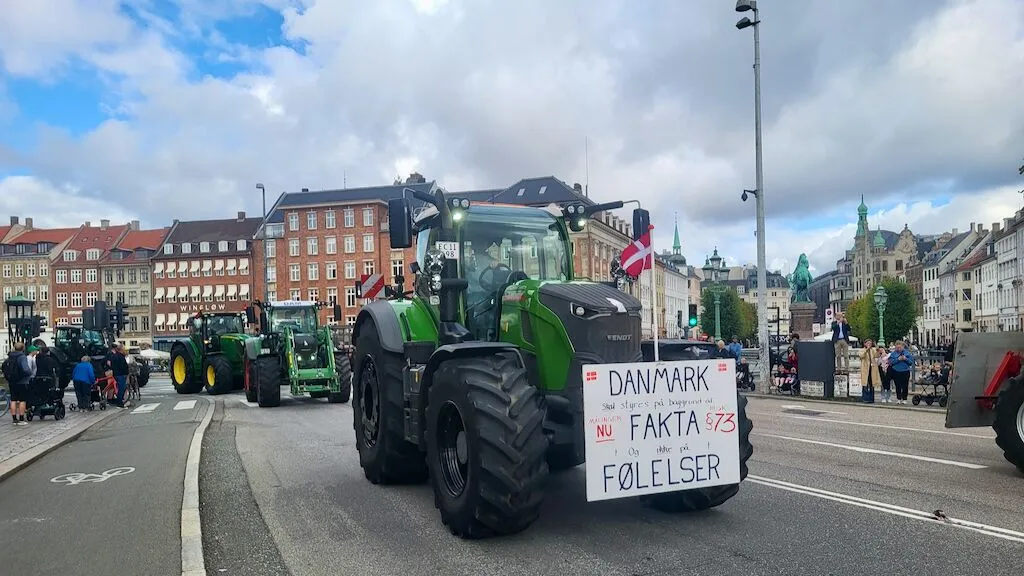
\includegraphics[width=0.45\textwidth]{pictures/traktor_kbh_3.jpeg}
\hspace{1em}
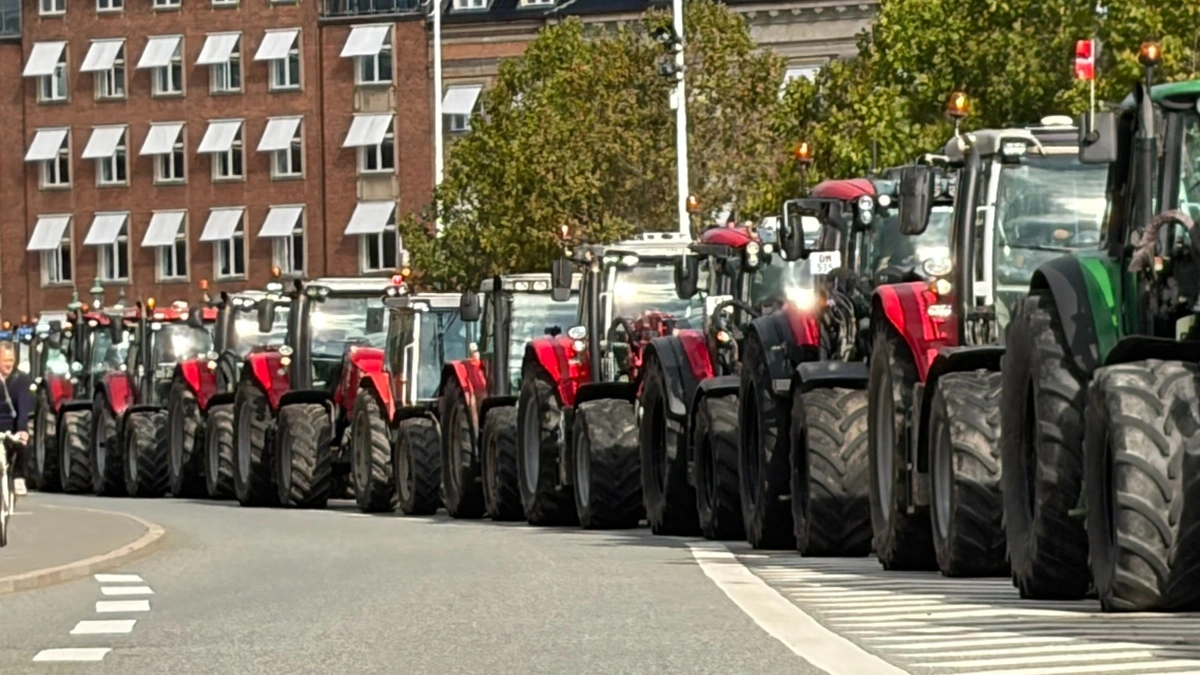
\includegraphics[width=0.45\textwidth]{pictures/traktor_kbh_4.jpeg}
\end{frame}


\begin{frame}[hvid]
\frametitle{\vspace{-3ex}Motivation: Data Requirements for Policy Design \& Impact Evaluation}

\begin{itemize}
\setlength{\itemsep}{1.5ex}
\item Various models are used to determine optimal policy implementations and their impacts  
\item These models require spatially explicit production and environmental data
\begin{itemize}
\setlength{\itemsep}{1ex}
\item Spatially explicit data on environmental externalities increasingly available
\item Lack of spatial explicit data on agricultural production and profitability\\
    $\Rightarrow$ most (all?) models and analyses are based on SEGES' planning data\\
    \quad (not based on real world, only 3 soil types, ignore climate, ignore field size/shape,\\
    \quad ignore unexplained variability, not independent)
\end{itemize}

\item We have developed a framework for estimating field-level data on input use, production and profitability based on existing real-world farm-level data

\item Combining this with existing environmental data,
we can asses field-level profitability from both the farmer's and society's perspective 
%\item Farm accountancy data + spatial environmental data
%\item DBII extended with nitrogen damage costs
\end{itemize}
\end{frame}


\begin{frame}[hvid]
\frametitle{\vspace{-3ex} Field-level Profitability -- Farmers' Perspective}
Profitability of a field from farmers' perspective
\begin{align*}
      = \frac{\text{field-level revenue} - \text{field-level variable costs}}{\text{field size}}
\end{align*}

\vspace{2ex}

We estimate this by:
\vspace{1.5ex}

\begin{itemize}
\setlength{\itemsep}{2.5ex}
\item Allocating input quantities (or costs) to production branches

\item Allocating output quantities (or revenues) to fields

\item Allocating production branch-specific input quantities (or costs) to fields
\end{itemize}
\end{frame}

% \begin{frame}[hvid]

% \frametitle{\vspace{-3ex}Methodology 1: Field-Level Profitability from Farmers' Perspective}
% Field-level profitability from farmers' perspective is estimated as:
% \begin{align*}
% \hat{\pi}^{\text{farmer}}_f = \big(\hat{y}_f - \hat{x}_f \big) / A_f
% \end{align*}

% \begin{itemize}

% \item $f = 1, \ldots, F =$ fields in the data set
% \vspace{1ex}

% \item $A_f =$ total area of field $f$
% \vspace{1ex}

% \item $\hat{y}_f =$ farmer's estimated total revenues of field $f$
% \vspace{1ex}

% \item $\hat{x}_f = \sum_p \hat{x}_f^p =$ farmer's estimated total costs of field $f$
% \vspace{1ex}

% \item $\hat{\pi}_f^{\text{farmer}} =$ farmer's estimated profitability of field $f$
% \end{itemize}

% \end{frame}


\begin{frame}[hvid]
\frametitle{\vspace{-3ex}Allocating Inputs to Production Branches}
\vspace{1ex}
\begin{itemize}
\setlength{\itemsep}{1.5ex}
\item Method is based on the `production branch statistics' of Danish farms (DST)
\vspace{1ex}
\begin{itemize}
    \item Bayesian estimation (priors, Stan)
\end{itemize}
\item We estimate how much of each farm's inputs (or costs) goes to each of its production branches, for example:
\end{itemize}
\vspace{3ex}
\centering
\begin{tikzpicture}[
    outerbox/.style={draw, minimum width=2.8cm, minimum height=3.3cm},
    font=\small
]
% Left box
\node[outerbox, fill=KUrod!10, align=center, font=\large] (total) {Total labour \\ costs};
% Right box (same height as left box), positioned closer
\node[outerbox, fill=KUrod!10, right=1.6cm of total] (right) {};
\node[font=\LARGE, black] at ($(total.east)!0.5!(right.west)$) {$\Rightarrow$};
\draw ($(right.north west)+(0,-0.825)$) -- ($(right.north east)+(0,-0.825)$);
\draw ($(right.north west)+(0,-1.65)$)  -- ($(right.north east)+(0,-1.65)$);
\draw ($(right.north west)+(0,-2.475)$) -- ($(right.north east)+(0,-2.475)$);
\node[align=center, font=\small] at ($(right.north)+(0,-0.4125)$) {Labour costs\\ for wheat};
\node[align=center, font=\small] at ($(right.north)+(0,-1.2375)$) {Labour costs\\ for spring barley};
\node[align=center, font=\small] at ($(right.north)+(0,-2.0625)$) {Labour costs\\ for dairy};
\node[align=center, font=\small] at ($(right.north)+(0,-2.8875)$) {\textit{etc.}};
\end{tikzpicture}
\end{frame}


% \begin{frame}[hvid]
% \frametitle{\vspace{-3ex}Total Input Use (1)}
% The empirical analysis is based on an accounting identity (Henningsen et al., 2026):
% \vspace{-1ex} \begin{align*}
%     x_i \equiv \sum_{j=1}^J \omega_{ij} A_{ij}
% \end{align*}

% \vspace{-1ex} \begin{itemize}
% \item $i = 1, \ldots, N =$ farm observation in the data set

% \item $j = 1, \ldots, J =$ production branch

% \item $x_i = $ farm $i$'s total quantity of a specific input in production

% \item $A_{ij} =$ farm $i$'s scope of production branch $j$ (e.g., hectare of wheat, units of cattle).

% \item $\omega_{ij} =$ farm $i$'s input-output coefficient in production branch $j$

% \item $\omega_{ij} A_{ij} = $ farm $i$'s quantity of input used in production branch $j$ (e.g., fertiliser per hectare of wheat)
% \vspace{1ex}

% \begin{itemize}
%         \item[\fontsize{12pt}{14pt}\selectfont $\rightarrow$]  Random coefficients ($\omega_{ij}$) addresses heteroscedasticity
%     \end{itemize}

% \end{itemize}

% \end{frame}



% \begin{frame}[hvid]
% \frametitle{\vspace{-3ex}Input Use per Unit of Production Branch (1)}
% We estimate individual input-output coefficients, assumed log-normally distributed:
% \begin{align*}
%         \omega_{ij} \sim \text{lognormal}\left(\beta_j+\sum_{m=1}^{M} \gamma_{jm} \, z_{mi}, \, \sigma_j^2 \right)
% \end{align*}
% \begin{itemize}
%     \item $m = 1, \ldots, M =$ factors that can affect input-output coefficients
%     \item $z_{im}:$ farm~$i$'s value of variables~$m$ (e.g., soil type, farm size, areas that can be irrigated, use of contractors, crop revenues, etc.)
%     \item $\beta_j$, $\gamma_{jm}:$ (hyper) parameters
%     \item $\sigma_j^2:$ variance parameter
%     \vspace{2ex}
    
%     \begin{itemize}
%         \item[\fontsize{12pt}{14pt}\selectfont $\rightarrow$]  Log-normal distribution ensures positive estimated coefficients
%     \end{itemize}
% \end{itemize}

% \end{frame}


% \begin{frame}[hvid]
% \frametitle{\vspace{-3ex} Bayesian Estimation (1)}

% \begin{itemize}
% \item Bayesian Markov-Chain Monte Carlo (MCMC) Estimation
% \vspace{1.5ex}
    
% \item ‘Stan’ platform \& language (through the R package ‘rstan’)
% \vspace{1.5ex}

% \item Priors:
% \vspace{1.5ex}

% \begin{itemize}
%     \item  Betas: $\beta_j \sim N \left( \text{mean}( \text{log}( \alpha_{j} ) ), \text{sd}( \text{log}( \alpha_{j} ) ) \right)$ \\ 
%     \vspace{1.5ex} 
    
%     where $\alpha_j$ are the estimated coefficients in 2024 obtained from the production branch statistics of Danish farms (DST).
%     \vspace{1.5ex}
    
%     \item  Gammas: $\gamma_{jm} \sim N( 0, \text{'rule-of-thumb'} )$ 
% \end{itemize}
% \vspace{1.5ex}

% \item Expected input-output coefficients is scaled relative to $\sigma_j$ so that: $\sum_{j=1}^J \tilde{\omega}_{ij} A_{ij} = x_i$
% \vspace{1.5ex}

% \begin{itemize}
%     \item[\fontsize{12pt}{14pt}\selectfont $\rightarrow$]  Bayesian setup with prior information addresses multicollinearity
% \end{itemize}
    
% \end{itemize}
% \end{frame}


%\begin{frame}[hvid]
%\frametitle{\vspace{-3ex} Obtaining Output-Specific Input Use (1)}

%\begin{itemize}
%    \item Parameters: $\beta_j$, $\gamma_{jm}$, $\sigma_j$

%    \vspace{-1ex} \begin{align*} E[ \omega_{ij} ] = \exp \left( \beta_j + \sum_{m=1}^M \gamma_{jm} z_{im} + \frac{\sigma_j}{2} \right)
%    \end{align*}

%    \item Farm $i$'s expected quantity of a specific input used in production branch $j$:
%    \vspace{-1ex} \begin{align*}
%    E[ \omega_{ij} A_{ij} ] = A_{ij} \exp \left( 
%    \beta_j + \sum_{m=1}^M \gamma_{jm} z_{im} + \frac{\sigma_j}{2}
%    \right)
%    \end{align*}

%    \item Expected input-output coefficients is scaled relative to $\sigma_j$ such that:
%    \vspace{-1ex} \begin{align*}
%    \sum_{j=1}^J \tilde{\omega}_{ij} A_{ij} = x_i \; \forall \; i    
%    \end{align*}
% \end{itemize}

% \end{frame}


\begin{frame}[hvid]
\frametitle{\vspace{-3ex} Allocating Outputs to Fields}

\vspace{-1ex}
\begin{itemize}
\setlength{\itemsep}{1.5ex}
\item We use a log-linear model to estimate each farm's revenue per hectare

\item Revenue per hectare at each field depends on field-level variables\\
(i.e., field size, crop sub-category, and soil type)

\item The observed total revenue of each crop category at each farm is allocated to all its fields on which the crop of the respective category is grown:
\end{itemize}

\vspace{1ex}
\centering
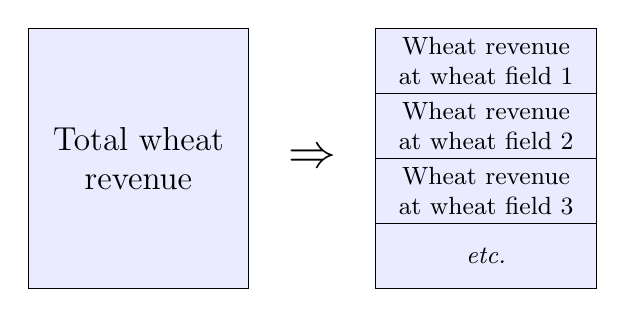
\begin{tikzpicture}[
    outerbox/.style={draw, minimum width=2.8cm, minimum height=3.3cm},
    font=\small
]
% Left box
\node[outerbox, fill=blue!8, align=center, font=\large] (total) {Total wheat\\revenue};
% Right box (same height as left box), positioned closer
\node[outerbox, fill=blue!8, right=1.6cm of total] (right) {};
\node[font=\LARGE, black] at ($(total.east)!0.5!(right.west)$) {$\Rightarrow$};
\draw ($(right.north west)+(0,-0.825)$) -- ($(right.north east)+(0,-0.825)$);
\draw ($(right.north west)+(0,-1.65)$)  -- ($(right.north east)+(0,-1.65)$);
\draw ($(right.north west)+(0,-2.475)$) -- ($(right.north east)+(0,-2.475)$);
\node[align=center, font=\small] at ($(right.north)+(0,-0.4125)$) {Wheat revenue \\at wheat field 1};
\node[align=center, font=\small] at ($(right.north)+(0,-1.2375)$) {Wheat revenue \\at wheat field 2};
\node[align=center, font=\small] at ($(right.north)+(0,-2.0625)$) {Wheat revenue \\at wheat field 3};
\node[align=center, font=\small] at ($(right.north)+(0,-2.8875)$) {\textit{etc.}};
\end{tikzpicture}
\end{frame}


\begin{frame}[hvid]
\frametitle{\vspace{-3ex}Allocating Inputs to Fields}

\vspace{-1ex}
\begin{itemize}
\setlength{\itemsep}{1.5ex}
\item We use the log-linear model to estimate each farm's costs per hectare

\item Costs per hectare depend on field-level variables (i.e., field size, crop, and soil type) and farm-level variables (i.e., farm size, areas that can be irrigated, crop revenues, applied nitrogen per hectare, and livestock units)

\item The total costs of each input and crop production branch at each farm (estimated in step~1) are allocated to fields, on which the crop is grown, for example:
\end{itemize}

\vspace{0.5ex}
\centering
\begin{tikzpicture}[
    outerbox/.style={draw, minimum width=2.8cm, minimum height=3.3cm},
    font=\small
]
% Left box
\node[outerbox, fill=KUrod!10, align=center, font=\large] (total) {Labour cost\\ for wheat};
% Right box (same height as left box), positioned closer
\node[outerbox, fill=KUrod!10, right=1.6cm of total] (right) {};
\node[font=\LARGE, black] at ($(total.east)!0.5!(right.west)$) {$\Rightarrow$};
\draw ($(right.north west)+(0,-0.825)$) -- ($(right.north east)+(0,-0.825)$);
\draw ($(right.north west)+(0,-1.65)$)  -- ($(right.north east)+(0,-1.65)$);
\draw ($(right.north west)+(0,-2.475)$) -- ($(right.north east)+(0,-2.475)$);
\node[align=center, font=\small] at ($(right.north)+(0,-0.4125)$) {Labour cost \\at wheat field 1};
\node[align=center, font=\small] at ($(right.north)+(0,-1.2375)$) {Labour cost \\at wheat field 2};
\node[align=center, font=\small] at ($(right.north)+(0,-2.0625)$) {Labour cost \\at wheat field 3};
\node[align=center, font=\small] at ($(right.north)+(0,-2.8875)$) {\textit{etc.}};
\end{tikzpicture}
\end{frame}


% \begin{frame}[hvid]
% \frametitle{\vspace{-3ex}Estimation Model: Outputs (2)}
% We estimate a log-linear model with farm fixed effects (to exploit variation within farms):
% \vspace{-2.5ex} \begin{align*}
%     \ln(y_{ik}/A_{ik}) = & \sum_{k'=1}^{K-1} \alpha_{k'} \mathbf{1}(k'=k) + \mu_1\,\text{fineshare}_{ik} + \mu_2\,\text{coarseshare}_{ik} \\
%     &+ \sum_{l=1}^{L} \rho_l\,\text{cropshare}_{il}\,D_{lk} 
%     + \lambda_i + \varepsilon_{ik}
% \end{align*}
% \vspace{-2ex}\begin{itemize}
%     \item $i = 1, \ldots, N =$ farm-crop observation; $k = 1, \ldots K =$ crop category; and $l = l, \ldots, L =$ crop sub-category
%     \item $\ln (y_{ik} / A_{ik}) =$ farm $i$'s (relative) average revenue per hectare of crop $k$
%     \item $\text{fineshare}_{ik}, \text{coarseshare}_{ik} =$ farm $i$’s shares of fine sandy and coarse sandy soils in production branch $j$ 
%     \item $\text{cropshare}_{lk} =$ crop $k$'s within-category share of crop sub-category $l$ (to account for different output-levels within crop categories)
% \end{itemize}

% \end{frame}



% \begin{frame}[hvid]
% \frametitle{\vspace{-3ex}Predicted Relative Revenues (2)}
% \begin{itemize}
% \item Based on the estimated the log-linear model we calculate predicted relative revenues ($\nu_{s(i,k,f),lk}$) associated with farm $i$'s soil type $s$ and crop category $k$
% \vspace{1.5ex}

% \item For example: For a farm $i$, cultivating wheat as the 'base' crop (K = wheat) on two fields f = 1, 2, where field 1 has fine sandy soil (s = 1) and field 2 has loamy soil (s = 3), and where all wheat is winter wheat, the predicted relative revenues are defined:
% \begin{align*}
%    \nu_{i1K} & = \exp(\lambda_i + \mu_1) \\[1ex]
%    \nu_{i3K} & = \exp(\lambda_i)
% \end{align*}
% \end{itemize}

% \end{frame}



% \begin{frame}[hvid]
% \frametitle{\vspace{-3ex}Allocating Field-level Outputs (2)}
% We allocate revenues to fields proportionally with field size and predicted relative revenues:
% \begin{align*}
%     \hat{y}_{ikf} = y_{ik} \cdot \frac{A_{ikf} \cdot \nu_{s(i,k,f),kl}}
%     {\sum_{f'=1}^{F_{ik}} A_{ikf'} \cdot \nu_{s(i,k,f'),kl}} 
% \end{align*}
% \vspace{-3ex} \begin{itemize}
%     \item $f = 1, \ldots, F$ indexes fields
%     \item $s(i,k,f) \in$ \{1 = fine sand, 2 = coarse sand, 3 = loamy soil\} is the predominant soil type on farm $i$'s field $f$ with crop $k$
%     \item $A_{ikf} =$ farm $i$'s observed area on field $f$ for crop category $k$
%     \item $\nu_{s(i,k,f),kl} =$ farm $i$'s predicted relative revenue with crop $k$ and crop sub-category $l$ 
%     \item $\hat{y}_{ikf} =$ farm $i$'s estimated revenue on field $f$ with crop $k$
%     \vspace{1ex}
%     \begin{itemize}
%     \item[\fontsize{12pt}{14pt}\selectfont $\rightarrow$]
%      Field-level allocation sum to the observed farm-level totals, and \\
%     \item[\fontsize{12pt}{14pt}\selectfont $\rightarrow$]
%      the allocation is driven by the soil type coefficients ($\mu_1, \mu_2$), i.e., crop-revenues respond identical to soil types
%     \end{itemize}
% \end{itemize}

% \end{frame}

\begin{frame}[hvid]
\frametitle{\vspace{-3ex}Data}

\begin{itemize}
\setlength{\itemsep}{1.5ex}
\item Sample of farms in Denmark (accountancy data from SEGES), 2024

\item Field-level (GIS) data, nitrogen retention and leaching maps

\item 23,336 fields cultivated by 894 conventional farms across eleven coastal catchments, and three aggregate soil types (fine sand, coarse sand, loamy soil)

\begin{itemize}
    \vspace{1.5ex}
    \item revenues: 12 output variables (wheat, barley, etc.)

    \vspace{1.5ex}
    \item costs: 10 input variables (labour, seed layout, fertiliser, etc.)

    \vspace{1.5ex}
    \item social costs: damages costs per kg nitrogen leaching to coastal waters, obtained from the literature (Andersen et al., 2019; Brink et al., 2011)

    % \item DB\,II$^\text{farmer}$: we present only catchment averages due to confidentiality concerns
    
    % \item DB\,II$^\text{society}$: both catchment averages and field-level estimates are presented since the reference scenario abstract from actual data
\end{itemize}

\end{itemize}
\end{frame}


\begin{frame}[hvid]
\frametitle{\vspace{-3ex} Results 1: Averages of Field-Level Revenues (Winter Wheat)}
\vspace{-1.6cm}
\centering
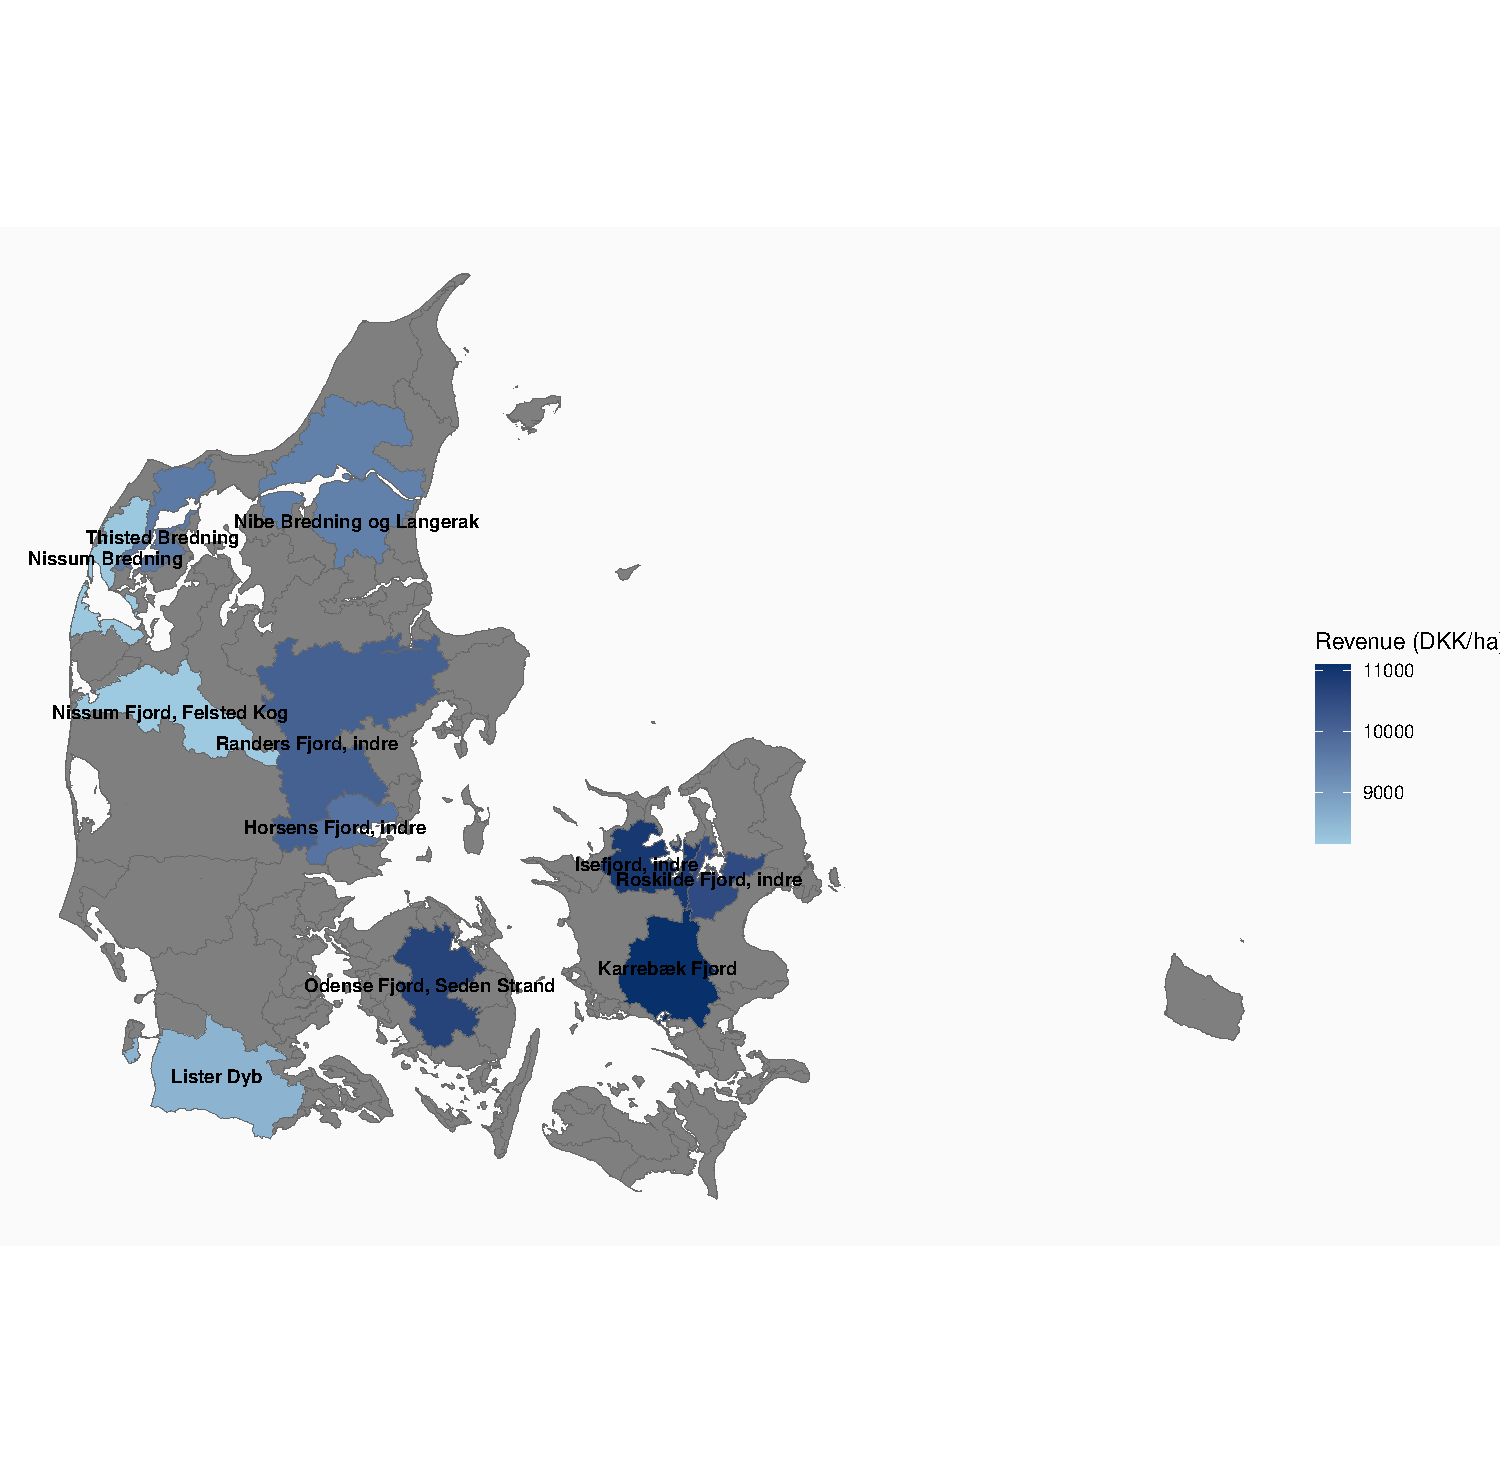
\includegraphics[width=\textwidth,height=1.2\textheight,keepaspectratio]{pictures/Revenue_wheat}
\end{frame}

\begin{frame}[hvid]
\frametitle{\vspace{-3ex} Results 1: Averages of Field-Level Costs (Winter Wheat)}
\vspace{-1.6cm}
\centering
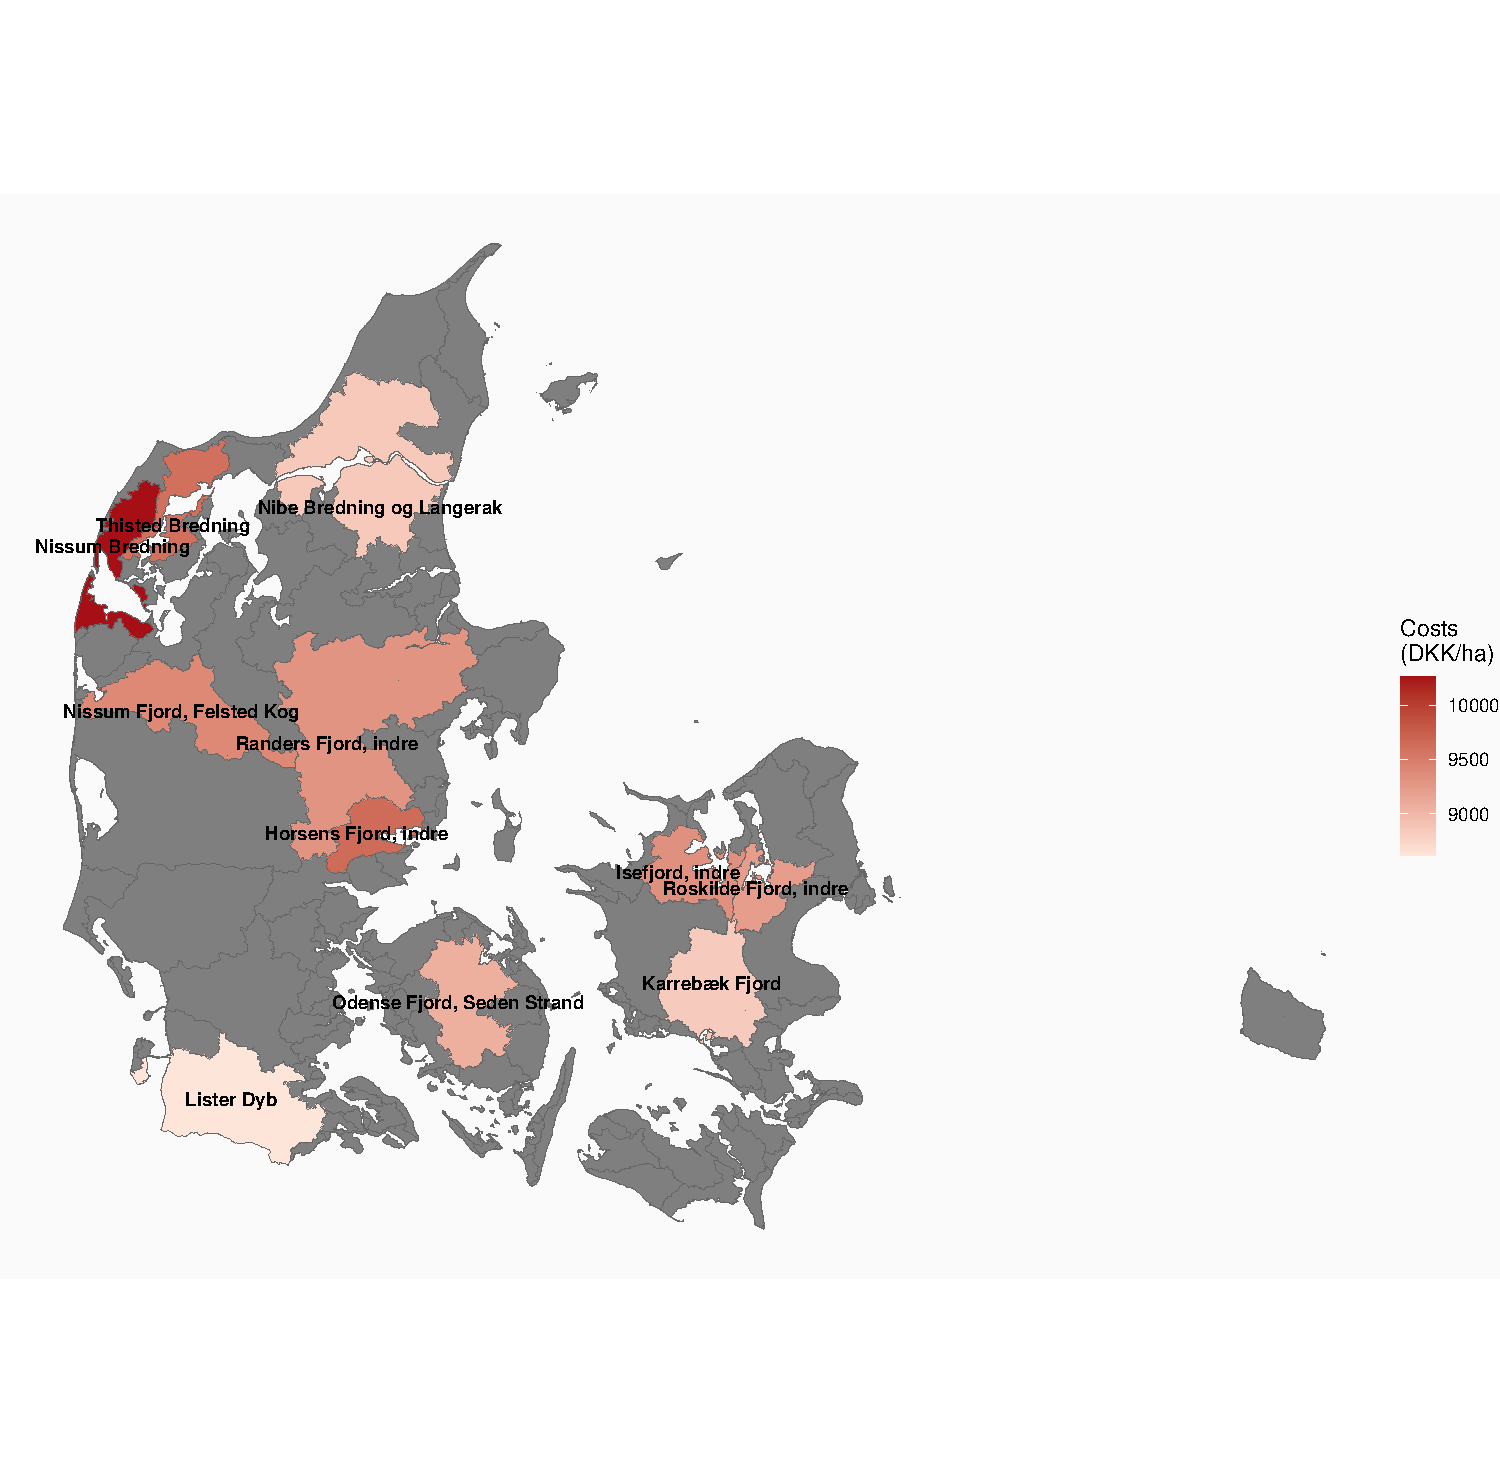
\includegraphics[width=\textwidth,height=1.2\textheight,keepaspectratio]{pictures/Costs_wheat.pdf}
\end{frame}


\begin{frame}[hvid]
\frametitle{\vspace{-3ex} Results 1: Averages of Field-Level Profitability (Winter Wheat)}
\vspace{-1.2cm}
\centering
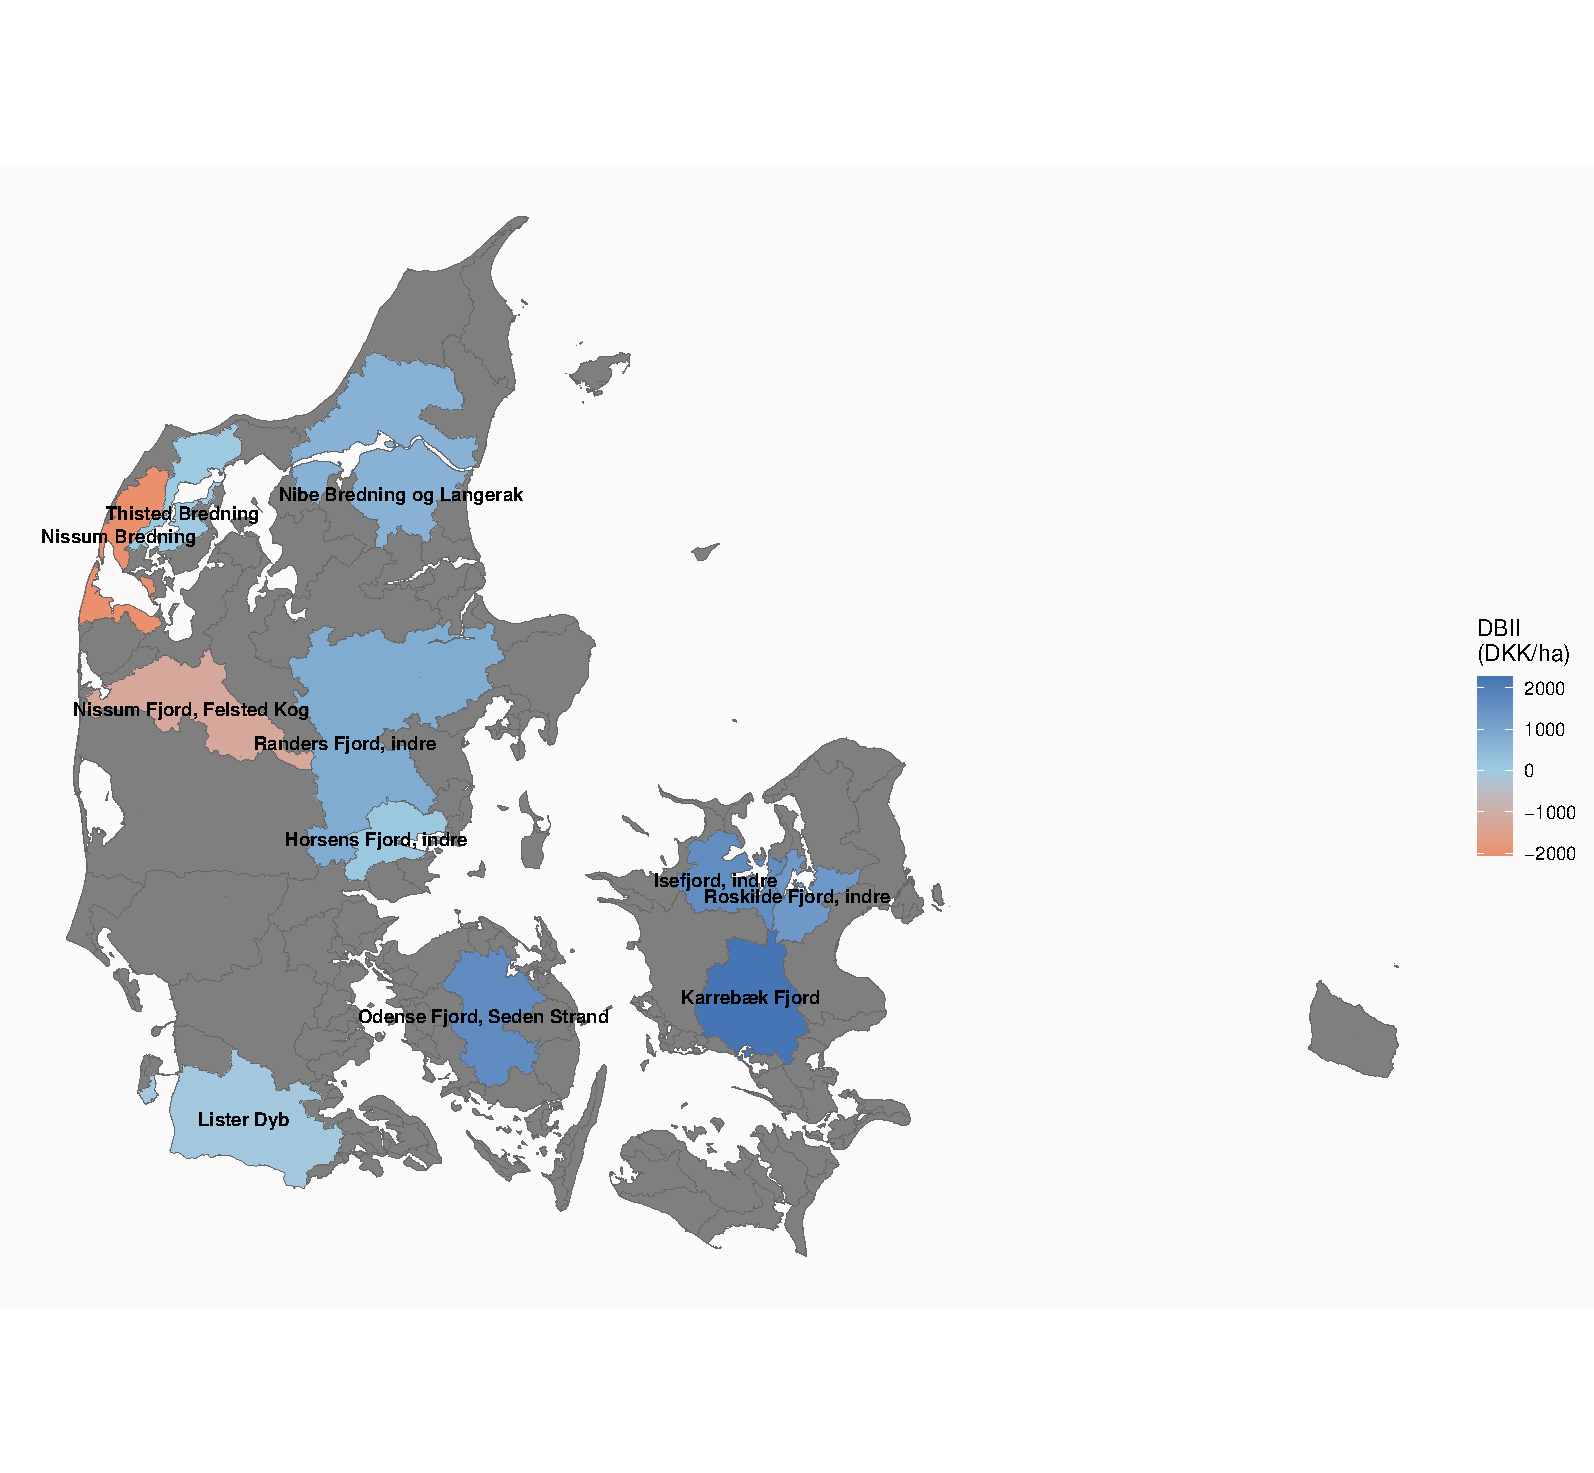
\includegraphics[
width=\textwidth,
height=1.2\textheight,
keepaspectratio
]{pictures/WW_prof.pdf}
\end{frame}


\begin{frame}[hvid]
\frametitle{\vspace{-3ex} Field-Level Profitability -- Society's Perspective}

Profitability of a field from society's perspective
\begin{align*}
      = \frac{\text{field-level revenue} - \text{field-level costs} \, \pm \, \text{societal valuation of field-level externalities}}{\text{field size}}
\end{align*}

\vspace{2ex}


We estimate this by:
\vspace{1.5ex}
\begin{itemize}
\setlength{\itemsep}{1.5ex}
   \item Using nitrogen leaching data based on a winter wheat reference scenario, and
   \item Estimating social damage costs associated with nitrogen leaching from individual fields
\end{itemize}
\end{frame}


\begin{frame}[hvid]
\frametitle{\vspace{-3ex}Winter Wheat Reference Scenario}

\begin{columns}[T]
\begin{column}{0.58\textwidth}
\begin{itemize}
    \item All fields are assumed to be cultivated with continuous winter wheat
    \item Fertilisation follows regulatory norms rather than actual farm management
    \item Each catchment: soil-type specific average DBII for winter wheat is used for all fields 
    \item Provides a consistent basis for comparing nitrogen leaching and profitability across fields
\end{itemize}
\end{column}

\begin{column}{0.38\textwidth}
    \centering
    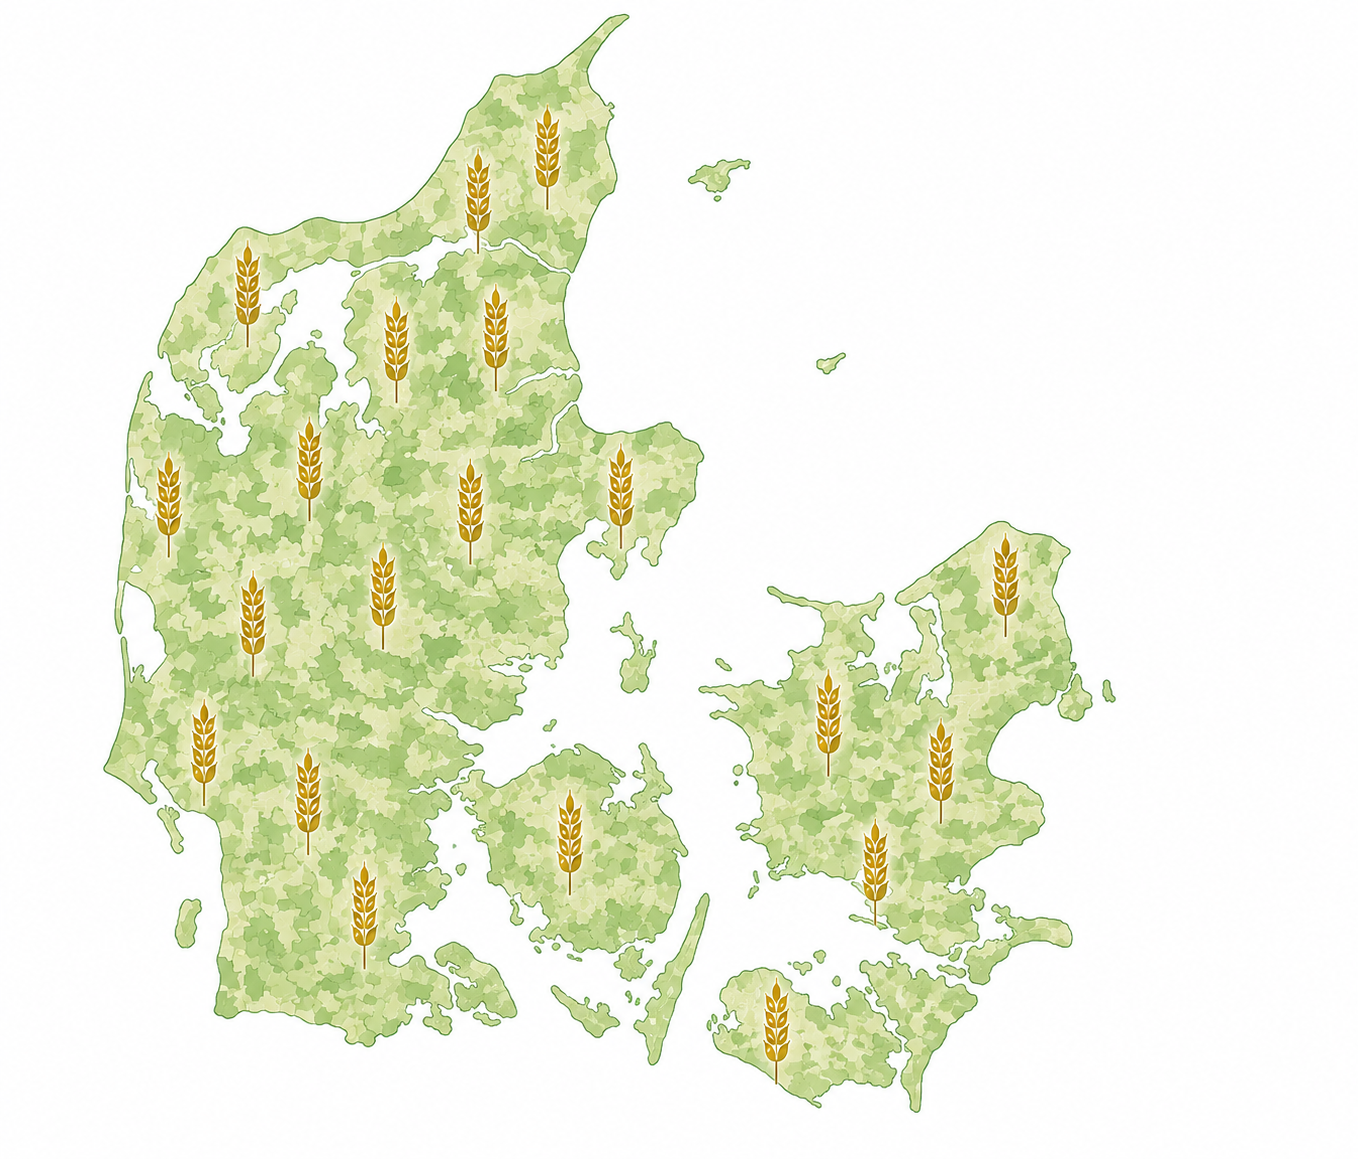
\includegraphics[
        width=\textwidth,
        height=0.68\textheight,
        keepaspectratio
    ]{pictures/hvedekort.png}
    \vspace{0.05cm}
    {\tiny Source: AI-generated with ChatGPT}
\end{column}
\end{columns}

\vspace{0.25cm}

%    \item\textbf{Removes variation from crop choice and farm management}

\textbf{Designed for field-level spatial comparison, not evaluation of field-level management}
\end{frame}

% \begin{frame}[hvid]
% \frametitle{\vspace{-3ex}Methodology (3): Field-Level Profitability from Society's Perspective}
% Field-level profitability from society's perspective under the winter wheat reference scenario is estimated as:
% \begin{align*}
    % \hat{\pi}_{f}^{\text{society,wheat}} = \bar{\pi}_{cs}^{\text{wheat}} - \hat{x}_{f}^{\text{society}}/A_{f}
% \end{align*}

% \vspace{1.5ex}
% \begin{itemize}
    % \item $s = 1, \ldots S =$ predominant soil type of field $f$
    % \vspace{1.5ex}
    
    % \item $c = 1, \ldots C =$ coastal catchment of field $f$
    % \vspace{1.5ex}
    
    % \item $\bar{\pi}_{cs}^{\text{wheat}} =$ estimated average profitability from winter wheat fields, with soil type $s$ \\ and catchment $c$
    % \vspace{1.5ex}

    % \item $\hat{x}_{f}^{\text{society}} =$ estimated  social damage costs of field $f$ associated with nitrogen leaching
    % \item $\hat{x}_{f}^{\text{society}}/A_{f} =$ estimated social damage cost per hectare of field $f$
    % \vspace{1ex}

    % \item If $\hat{\pi}_f^{\text{society,wheat}} > 0$ the field generates a net positive value from society’s perspective; $\hat{\pi}_f^{\text{society,wheat}} < 0$ indicates that the environmental damage costs exceed farmer returns
    
% \end{itemize}

% \end{frame}

\begin{frame}[hvid]

\frametitle{\vspace{-3ex}Field-Level Social Damage Costs}
We estimate field-level social damage costs associated with nitrogen leaching as:
\vspace{1ex}
\begin{align*}
    Social \, Cost_i & =  N^{\text{coast}}_i  \cdot SDC_{c(i)}\\
    & = \left( N^{\text{leached}}_i \cdot \left(1 - N^{\text{retention}}_i\right) \cdot Area_i \right) \cdot SDC_{c(i)}
\end{align*}
\vspace{-3ex}

With:
\begin{itemize}
\setlength{\itemsep}{1ex}
\item $N^{\text{coast}}_i$ = total quantity of nitrogen reaching coastal waters from field~$i$

\item $N^{\text{leached}}_i$ = quantity of nitrogen per hectare leached on field~$i$

\item $N^{\text{retention}}_i \in [0,1]$ = nitrogen retention rate of field~$i$ % indicating losses during transport from the field to coastal waters

\item $Area_i$ = size of field~$i$ [ha]

\item $SDC_{c(i)} =$ social damage cost per kg of nitrogen reaching coastal waters\\
\qquad\qquad of catchment~$c$, in which field~$i$ is located
\end{itemize}
\end{frame}


\begin{frame}{\vspace{-3ex} Social Damage Costs (SDC)}


From \textbf{Andersen et al. (2019)} - available for 6/11 Catchments
\begin{itemize}
    \vspace{1.5ex}
    \item Links reduction in N loadings to coastal waters with water clarity and economic benefits
    \vspace{1.5ex}
    \item Based on old baseline (2010) and (uniform) WFD reduction targets
    \vspace{1.5ex}
    \item Relies on benefit transfers from studies linking improved water quality to economic benefits (e.g., recreation and property prices but not biodiversity)
    \vspace{1.5ex}
    \item Densely populated and high-income areas lead \textit{ceteris paribus} to higher SDC 
\vspace{1ex}
    
\end{itemize}

%\vspace{0.2cm}

\begin{alertblock}{}
\centering
\textbf{Best available SDC for capturing relative spatial differences,\\
but substantial uncertainty in the absolute SDC values.}
\end{alertblock}

\end{frame}


\begin{frame}{\vspace{-3ex} Social Damage Cost Estimates}

\vspace{-2ex}
\begin{table}[htbp]
\centering
\small
\caption{Damage Cost Estimates}
\label{tab:damage-costs}
\begin{threeparttable}
\begin{tabular}{lrr}
\toprule
Coastal Catchment & DKK/kg N \\
\midrule
Roskilde Fjord, indre   & 74.34  \\
Odense Fjord, Seden Str.& 44.04  \\
Horsens Fjord, indre    & 87.80  \\
Nissum Fjord, Felsted Kog& 11.99  \\
Randers Fjord, indre    & 21.93  \\
Isefjord, indre         & 69.34  \\
\midrule
European Nitrogen Assessment           & [52.30--209.21] \\
\bottomrule
\end{tabular}
\begin{tablenotes}
\footnotesize
\small
\item 
Table reflects 2024 prices.
\end{tablenotes}
\end{threeparttable}
\end{table}

\end{frame}





%\begin{frame}[hvid]

%\frametitle{\vspace{-3ex}Allocating Outputs to Fields}

%\begin{itemize}
%\item For each type of crop, the total revenue is allocated to all fields on which the crop is grown
%\vspace{1.5ex}
    
%\item The sum of estimated amounts over all fields must be equal to the observed amount at the farm
%\vspace{1.5ex}
    
%\item Revenue per hectare at each field can depend on:
%\vspace{1ex}
    
%\begin{itemize}
%    \item Field-level variables (e.g., soil type, geographical location, ...)
%    \vspace{1ex}
        
%    \item Farm-level variables (e.g., amounts of organic manure per hectare, ...)
% \end{itemize}

% \end{itemize}

% \end{frame}


% \begin{frame}{\vspace{-3ex} Results (1): From Farmer to Social Profitability}

% \begin{table}[H]
% \centering
% \small
% \caption{Average field-level profitability and nitrogen damage costs (DKK/ha/y)}
% \label{tab:defence_summary}
% \begin{tabular}{lrrrrr}
% \toprule
% \textbf{Catchment}
% &
% \textbf{DBII$^{farmer}$}
% &
% \textbf{Specific}
% &
% \textbf{DBII$^{soc}$}
% &
% \textbf{Uniform}
% &
% \textbf{DBII$^{soc}$}
% \\
% &
% &
% \textbf{Damage}
% &
% \textbf{(Specific)}
% &
% \textbf{Damage}
% &
% \textbf{(Uniform)}
% \\
% \midrule
% Nissum Fjord
% & -1,238
% & 251
% & -1,476
% & 2,325
% & -3,512
% \\

% Randers Fjord
% & 783
% & 315
% & 466
% & 1,595
% & -799
% \\

% Horsens Fjord
% & 86
% & 1,649
% & -1,567
% & 2,086
% & -2,003
% \\

% Odense Fjord
% & 1,637
% & 732
% & 895
% & 1,845
% & -220
% \\

% Isefjord
% & 1,597
% & 1,105
% & 539
% & 1,770
% & -126
% \\

% Roskilde Fjord
% & 1,304
% & 679
% & 811
% & 1,014
% & 501
% \\

% \bottomrule
% \end{tabular}
% \end{table}

% \end{frame}

%\begin{frame}{\vspace{-3ex}Results (2): The Valuation Approach Changes Relative Priorities}

%\begin{table}
%\centering
%\small
%\caption*{Area-weighted average nitrogen damage costs (DKK/ha)}
%\begin{tabular}{lccc}
%\toprule
%\textbf{Catchment}
%&
%\textbf{SDC (Specific)}
%&
%\textbf{Specific}
%&
%\textbf{Uniform}
%\\
%\midrule

%Nissum Fjord, Felsted Kog
%& 11.99
%& 251 (1)
%& 2,325 (6)
%\\

%Randers Fjord, indre
%& 21.93
%& 315 (2)
%& 1,595 (2)
%\\

%Roskilde Fjord, indre
%& 74.34
%& 679 (3)
%& 1,014 (1)
%\\

%Odense Fjord, Seden Strand
%& 44.04
%& 732 (4)
%& 1,845 (4)
%\\

%Isefjord, indre
%& 69.34
%& 1,105 (5)
%& 1,770 (3)
%\\

%Horsens Fjord, indre
%& 87.80
%& 1,649 (6)
%& 2,086 (5)
%\\

%\bottomrule
%\multicolumn{4}{l}{\footnotesize Rank in parentheses (1 = lowest damage cost). SDC (Uniform) = 130.76 DKK/Kg N}
%\end{tabular}
%\end{table}

%\begin{itemize}
%    \item The following considers DBII$^{society}$ based on the specific valuation approach
%\end{itemize}
%\end{frame}

\begin{frame}[hvid]
\frametitle{\vspace{-3ex} Results 2: Field-Level Profitability -- Society's Perspective}

\centering
\includegraphics[width=\textwidth,height=0.8\textheight,keepaspectratio]{pictures/hist_specific_DBII_hvede.pdf}

\end{frame}

\begin{frame}[hvid]
\frametitle{\vspace{-3ex}Results 2: Average Field-Level Profitability -- Society's Perspective}
\vspace{-1.6cm}
\centering
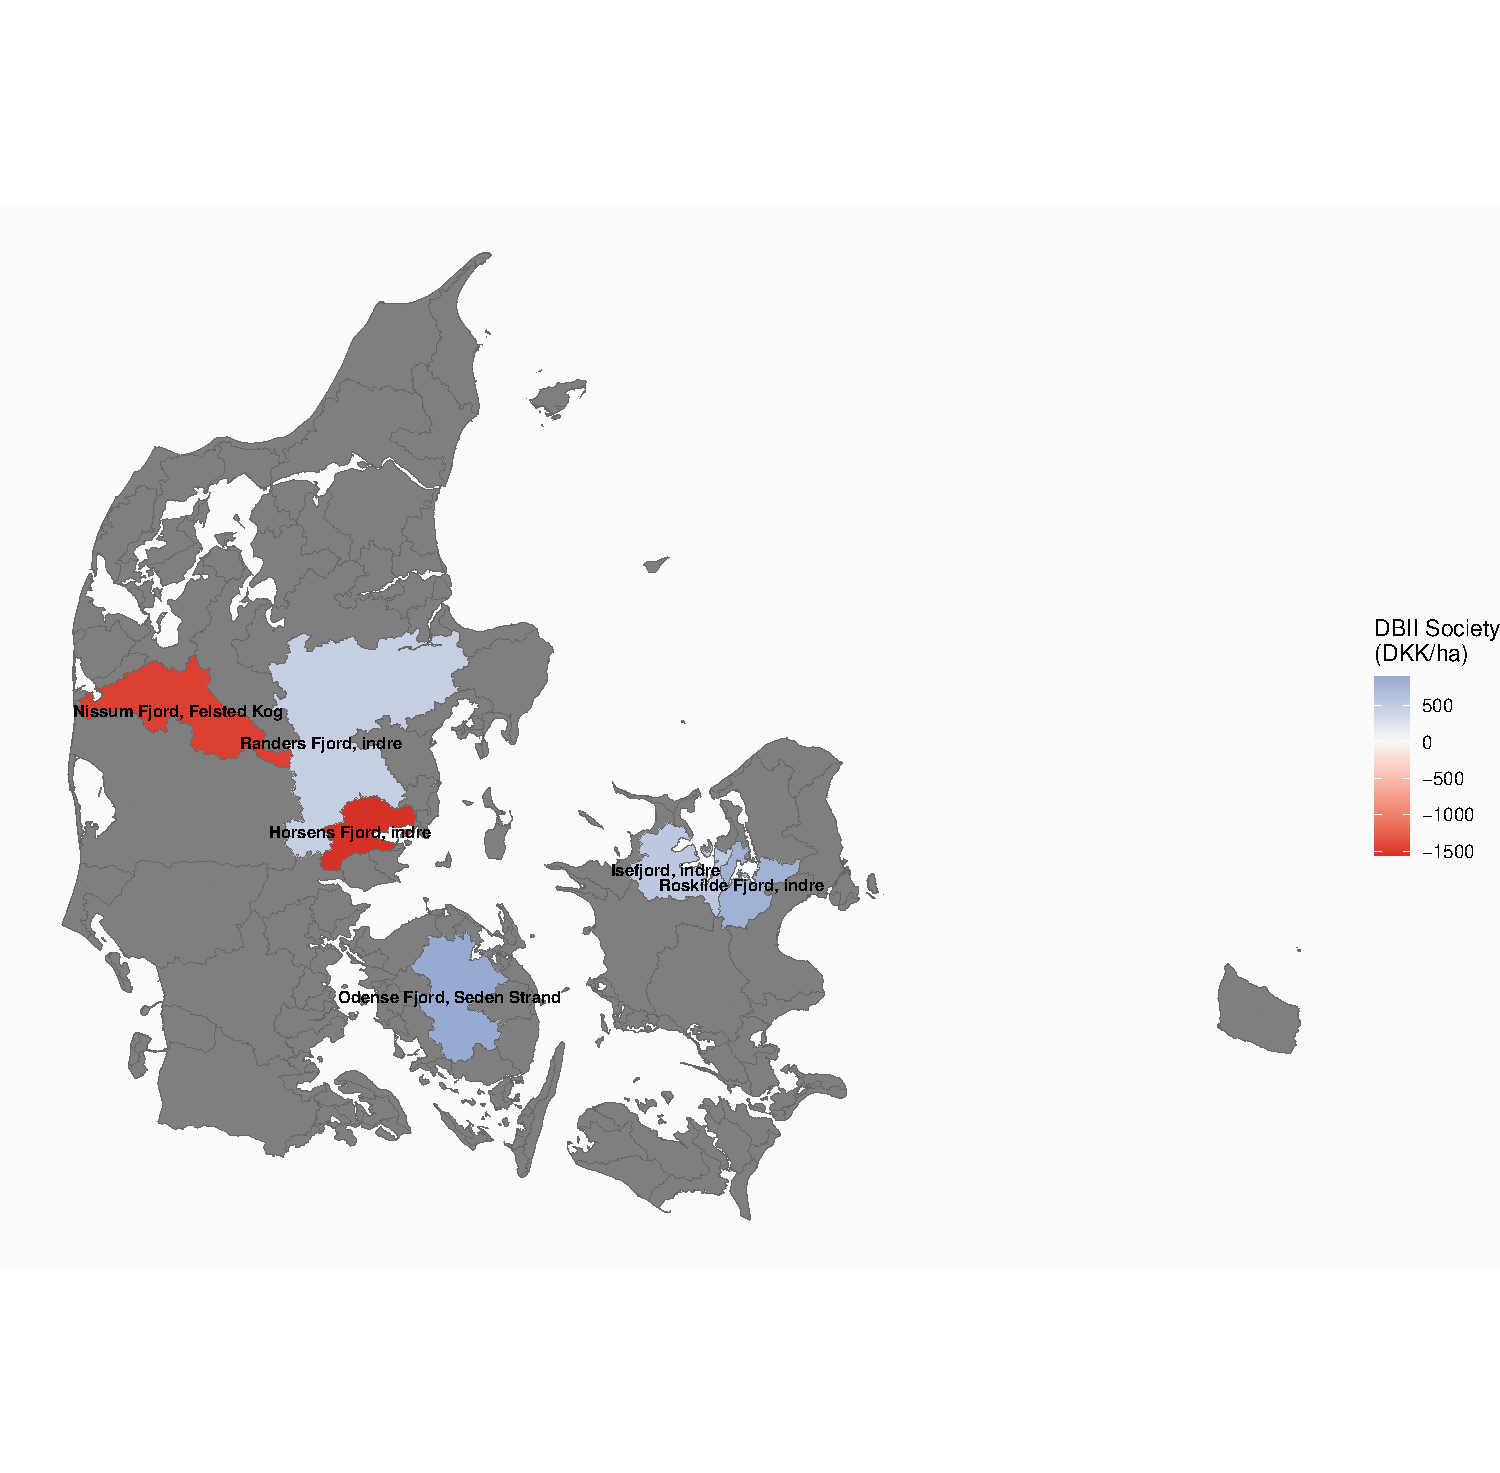
\includegraphics[width=\textwidth,height=1.2\textheight,keepaspectratio]{pictures/DBII_SOC_SPEC.pdf}

\end{frame}


\begin{frame}{\vspace{-3ex}Results 2: What Drives Profitability from Society's Perspective?}

\vspace{-2ex} \begin{table}
\centering
\small
\caption{Average field-level profitability and social costs (DKK/ha)}
\begin{tabular}{lrrr}
\toprule
\textbf{Catchment}
&
\textbf{Farmer}
&
\textbf{Social costs}
&
\textbf{Society}
\\
\midrule

Randers Fjord, indre
& 783
& 315
& 466
\\

Horsens Fjord, indre
& 86
& 1,649
& -1,567
\\

Isefjord, indre
& 1,597
& 1,105
& 539
\\

\bottomrule
\end{tabular}
\end{table}



\begin{itemize}
    \item Randers Fjord, indre: moderate farmer profitability and low social costs \\ $\rightarrow$ socially profitable
    \item Horsens Fjord, indre: quite low farmer profitability but high social costs 
    \\ $\rightarrow$ socially unprofitable
    \item Isefjord, indre: high farmer profitability offsets substantial social costs
\end{itemize}
\vspace{1ex}


\centering
\textbf{Field-level profitability from society's perspective depends on both farmers' profitability and environmental damages from nitrogen leaching.}


\end{frame}




\begin{frame}[hvid]
\frametitle{\vspace{-3ex}Main Findings}

\begin{enumerate}
\setlength{\itemsep}{1.5ex}
\item Field-level profitability from farmer's perspective varies substantially across catchments and also across fields within the same catchment

\item Environmental damages (costs) vary substantially across catchments and also across fields within the same catchment

\item Field-level profitability from society's perspective depends on the difference between the two
\end{enumerate}
\vspace{5ex}

\centering
\textbf{Profitability can be estimated at the field level both from farmers' and society's perspective -- appropriate damage cost estimates are needed}

\vspace{4ex}

%\textbf{Key Takeaway:} Neither profitability nor environmental damages alone identify the fields where intervention yields the greatest gains for society.

\end{frame}




%\begin{frame}[hvid]
%\frametitle{\vspace{-3ex}Discussion}

%\begin{itemize}
%\item[1.] Methodological challenges
%\vspace{1.5ex}

%\item[2.] Robustness check
%\vspace{1.5ex}

%\item[2.] Social damage costs (SDC)


%\end{frame}

% \begin{frame}[hvid]
% \frametitle{\vspace{-3ex}Discussion: Measuring Social Profitability Requires Trade-offs}

% \vspace{-1ex} \begin{itemize}

% \item Reference Scenario
% \vspace{1ex}

% \begin{itemize}
%     \item[$+$] Comparability across fields
%     \vspace{1ex}
    
%     \item[$-$] Does not capture realised management
% \end{itemize}
% \vspace{1ex}

% \item Average Field-Level Profitability (DBII)
% \vspace{1ex}
% \begin{itemize}
%     \item[$+$] Consistent and tractable framework
%     \vspace{1ex}
    
%     \item[$-$] Ignores within-group profitability variation
% \end{itemize}
% \vspace{1ex}

% \item Specific Damage Costs
% \vspace{1ex}

% \begin{itemize}
%     \item[$+$] Reflect local environmental conditions
%     \vspace{1ex}
    
%     \item[$-$] Available for only six catchments
% \end{itemize}
% \vspace{1ex}
% \end{itemize}

% \small
% \centering
% \textbf{The framework priorities comparability and spatial consistency over field-level precision.}

% \end{frame}


%  \begin{frame}[hvid]
%\frametitle{\vspace{-3ex}Discussion (1): Methodological Challenges}

%\vspace{-1.5ex} \begin{itemize}

%\item Model specification with interaction terms and farm fixed effects
%\vspace{1ex}

%\begin{itemize}
%    \small
 %   \item[$+$] Statistically favoured (Waldtest) $\rightarrow$ soil type effects likely different across crop categories
  %  \vspace{1ex}
   % \item[$-$] Produces agronomically implausible estimates
    %\vspace{1ex}
%\end{itemize}

%\item Model specification without interaction terms and with farm fixed effects
%\vspace{1ex}

%\begin{itemize}
 %   \small
 %   \item[$+$] Produces agronomically plausible estimates %$\rightarrow$ lower revenues relative to loamy soil
 %   \vspace{1ex}
 %   \item[$-$] Not favoured statistically
 %   \vspace{1ex}
%\end{itemize}

%\item No estimated soil type coefficient is statistically significant. Potential reasons:
%\vspace{1ex}
%\begin{itemize}
 %   \item Three broad soil type groups may obscure finer soil variation available to the model
 %   \vspace{1ex}
  %  \item Only a single year of data (farm fixed effects may absorb some within-farm variation in soil type composition)
 %   \vspace{1ex}
    % \item Farmers may adapt management practices to local soil type conditions \textcolor{KUrod}{$\rightarrow$}
    % may partly offset differences in revenues across soil types
% \end{itemize}

% \end{itemize}

%\small
%\centering
%\textbf{Using multiple years and more disaggregated soil types may provide more within-farm variation over time and a more precise identification of soil type effects}

%\end{frame}



% \begin{frame}[hvid]
% \frametitle{\vspace{-3ex}Discussion (2): Reference Scenario}

% \begin{itemize}

% \item Actual Management
% \vspace{1ex}

% \begin{itemize}
%     \item[$+$] Reflects realised nitrogen losses
%     \vspace{1ex}
    
%     \item[$-$] Results depend on current management choices
% \end{itemize}
% \vspace{1ex}

% \item Reference Scenario
% \vspace{1ex}

% \begin{itemize}
%     \item[$+$] Evaluates the underlying environmental vulnerability of the field
%     \vspace{1ex}
    
%     \item[$+$] Provides a consistent basis for comparison across fields
%     \vspace{1ex}
    
%     \item[$-$] Does not capture realised management practices
% \end{itemize}
% \vspace{1ex}

% \item Policy Perspective 
% \vspace{1ex}

% \begin{itemize}
%     \item Long term spatial targeting should be based on field characteristics rather than temporary management decisions: \textbf{Evaluate the field, not the farmer}
% \end{itemize} 

% \end{itemize}


% \end{frame}

%\begin{frame}[hvid]
%\frametitle{\vspace{-3ex}D%iscussion (2): Robustness %Check}


%\begin{itemize}

%\item DBII (spring barley)
%\vspace{1ex}
%\begin{itemize}
%\item DBII for spring barley does not show same geographic pattern (west-east gradient) 
%\vspace{1ex}

%\item DBII for spring barley is unprofitable for all catchments
%\vspace{1ex}

%\item Revenues for spring barley is lower (on average) compared to DST figures
%\end{itemize}
%\vspace{1ex}

%\item Reference crop (spring barley with catch crop following spring barley) 
%\vspace{1ex}

%\begin{itemize}
%\item Relative catchment rankings are largely preserved
%\vspace{1ex}

%\item Absolute damage costs are sensitive to crop reference choice (catch-crop effect)
%\vspace{1ex}

%\item Different spatial resolution on reference maps 
%\vspace{1ex}

%\item Evaluated at catchment level only

%\end{itemize}
%\vspace{1ex}

%\end{itemize}

%\item Crop Allocation
%\vspace{1ex}

%\begin{itemize}
%\item[$+$] No evidence of systematic crop sorting by environmental burden
%\vspace{1ex}

%\item[$-$] Evaluated at catchment level only
%\end{itemize}
%\vspace{1ex}
%\end{itemize}
%\vspace{1ex}

%\small

%\centering
%\textbf{The robustness check is indicative at best, and should be investigated more thoroughly} 

%\end{frame}


%\begin{frame}[hvid]
%\frametitle{\vspace{-3ex}Future Research}

%\vspace{-1ex}\begin{itemize}

%\item Data
%\vspace{1ex}

%\begin{itemize}
%\item Panel data set with multiple years to investigate growth in field-level profitability
%\vspace{1ex}

%\item Representative sample of farms (e.g., national sample)
%\end{itemize}
%\vspace{1ex}

%\item Profitability Estimates
%\vspace{1ex}

%\begin{itemize}
%\item More appropriate field-level DBII estimates
%\vspace{1ex}

%\item More detailed soil type classification
%\end{itemize}
%\vspace{1ex}

%\item Environment
%\vspace{1ex}

%\begin{itemize}
%\item Updated Danish damage costs
%\vspace{1ex}

%\item Additional externalities (e.g., groundwater leaching, or biodiversity improvements)

%\end{itemize}

%\end{itemize}

%\vspace{1.5ex}

%\small 
%\centering
%\textbf{The framework should be viewed as a proof of concept.}\
%\textbf{The next step is to improve the quality and spatial resolution of the underlying inputs / costs.}

%\end{frame}


%\begin{frame}[hvid]
%\frametitle{\vspace{-3ex} Future Improvements (1): Approximation of DBII}
%\begin{itemize}
%\item Individual field-level estimates are likely infeasible due to statistical noise and limited data availability (SEGES relies on voluntary participation)
%\vspace{1.5ex}

%\item Some level of spatial approximation is necessary
%\vspace{1.5ex}

%\item However, the appropriate geographical basis for approximation is not clear
%\vspace{1.5ex}
  
%\end{itemize}

%\end{frame}



%\begin{frame}[hvid]
%\frametitle{\vspace{-3ex} Future Improvements (1): Approximation of DBII}

%\begin{itemize}

%\item The current catchment-level approximation of DBII may not be appropriate
%\vspace{1.5ex}
    
%\begin{itemize}
%    \item Adjacent and otherwise similar fields may receive different DBII values due to arbitrary catchment boundaries
%    \vspace{1.5ex}
    
%    \item Farmers with fields located in multiple catchments may face different DBII values across otherwise comparable fields    
%    \vspace{1.5ex}
%\end{itemize}

%\item Explore panel data to identify more appropriate approximation basis
%\vspace{1.5ex}
    
%\begin{itemize}
%    \item Identify meaningful spatial groupings based on profitability patterns in multi-year data
%    \vspace{1.5ex}
    
%    \item Aim to develop a more data-driven and less arbitrary spatial approximation 
%    \vspace{1.5ex}
%\end{itemize}

%\end{itemize}

% \end{frame}






%\begin{frame}[hvid]
%\frametitle{\vspace{-3ex}Social Damage Costs}
%\begin{itemize}
%\item Why does the choice of social damage cost matter?
%\item Environmental damages are inherently spatially differentiated
%\vspace{1.5ex}
%\begin{itemize}
%\item Biophysical impacts differ across water bodies (e.g. Limfjorden, Lillebælt, and the North Sea)
%\item Social benefits from environmental improvements may also differ due to variation in recreational use and willingness-to-pay
%\end{itemize}
%\vspace{1.5ex}
%\item No valuation approach is value-free
%\vspace{1.5ex}
%\begin{itemize}
%\item Ignoring social damage costs is a normative choice 
%\item Willingness-to-pay measures involve distributional considerations
%\item Cost-based approaches involve implicit value judgments
%\item Political targets and priorities are normative by nature
%\end{itemize}
%\item The challenge is therefore not to eliminate normativity, but to make assumptions explicit and policy choices transparent

%\end{itemize}
%\end{frame}


\begin{frame}[hvid]
\frametitle{\vspace{-3ex}  Future Improvements}

\vspace{-1ex}
Current Scope: Pilot framework
(nitrogen externalities only,
based on a single year of data)
\vspace{1ex}

Future Scope
\begin{itemize}
\setlength{\itemsep}{1ex}
\item Connecting the estimations of inputs/costs per field and outputs/revenues per field%Revenue per hectare may depend on farm-level variables (e.g., amount of fertiliser per hectare)

\item Panel data with multiple years 
(more precise estimates; more representative)  %(e.g., data set grows each year, or `rolling window')

\item Averages over multiple years and/or crop rotations

\item Data from all available farms in all catchments

\item Including also organic farms (accounting for differences)

\item Additional externalities (e.g., GHG emissions, pesticides, and biodiversity)

\item Develop method for estimating input use directly from farm-level to field-level 

\item Including additional data (e.g., satellite data on biomass per ha)
\end{itemize}
\end{frame}


\begin{frame}[hvid]
\frametitle{\vspace{-3ex}Conclusions}
\vspace{-2ex}
\begin{itemize}
\setlength{\itemsep}{1ex}
\item We can estimate field-level inputs/costs, yields/revenues, and profitability based on real-world data.

\item Extending this small pilot project (MSc project) to a research project with multiple researchers and much more data $\rightarrow$ improve accuracy, representativeness, and coverage
\end{itemize}
\vspace{1.5ex}

\textbf{Why should we do this?}
\begin{itemize}
\setlength{\itemsep}{1ex}
\item Green Tripartite Agreement, Agri-Environmental Schemes, \ldots
\begin{itemize}
    \setlength{\itemsep}{1ex}
    \item Identify fields where environmental benefits of retirement exceed forgone agricultural value

    \item Identify fields where continued agricultural production remains socially beneficial

    \item Directing subsidies/interventions to fields or areas, where social returns are highest %Spatially targeted schemes based on societal benefits
    
   % \item "Windfall gains" become less problematic ("reward" socially desirable management)
\end{itemize}
\item Use of more accurate real-world based field-level data on input use, production, and profitability in many models and analyses\\
$\rightarrow$ more effective and efficient regulation, more reliable estimates of impacts
\end{itemize}
\end{frame}



\begin{comment}
\begin{frame}[hvid]
\frametitle{\vspace{-3ex}Corrections}
\begin{itemize}
    \item p 25: in Table 2 the number of organic farms excluded is 119 (not 134)
    \item Catchments presentet are NOT ID15 (but broader VP3 classifications)
    \item p 25: Nissum Fjord, Feldsted Kog not mentioned
    \item p 28: wrong reference Table 3 (not 19)
    \item p 30: table reference left out (Table 23)
    \item p 32: table reference should have appendix reference
    \item p 32: farmer profitability - not social profitability
    \item p 98: we exclude the share of loamy soil (\textit{JB 5 and 6 lerjord}), not coarse sand.
    \item p 106: Table 23 should have bullet points for livestock production branches at LUs
\end{itemize}
\end{frame}
\end{comment}


\begin{frame}[hvid]
\frametitle{\vspace{-3ex}A. Data: Crop Composition of Output Data Set}

\begin{table}[H]
\centering
\small
\begin{tabular}{lrrr}
\toprule
\textbf{Crop category} & \textbf{Farm-crop Obs.} & \textbf{Crop area (ha)} & \textbf{Avg.\ revenue per hectare} \\
\midrule
Barley              &   719 & 54{,}808 &  6{,}927 \\
Wheat               &   627 & 44{,}947 &  9{,}663 \\
Rapeseed            &   475 & 19{,}018 & 12{,}825 \\
Fodder maize        &   303 & 26{,}479 &  9{,}516 \\
Rye/Triticale       &   295 & 10{,}230 &  8{,}112 \\
Roughage            &   282 & 26{,}211 &  3{,}176 \\
Seeds               &   169 &  6{,}318 & 11{,}461 \\
Oats/Mixed grain    &   129 &  3{,}283 &  7{,}775 \\
Potatoes            &   105 &  7{,}907 & 61{,}492 \\
Legumes             &    74 &  2{,}010 &  8{,}659 \\
Sugar beet          &    42 &  1{,}235 & 18{,}663 \\
Energy crops        &    12 &    180   & 20{,}079 \\
\midrule
\textbf{Total}      & \textbf{3{,}232} & \textbf{202{,}628} & $-$ \\
\bottomrule
\end{tabular}
\end{table}

\end{frame}


\begin{frame}[hvid]
\frametitle{\vspace{-3ex}B. Methodology: Total Input Use}
The empirical analysis is based on an accounting identity (Henningsen et al., 2026):
\vspace{-1ex} \begin{align*}
    x_i \equiv \sum_{j=1}^J \omega_{ij} A_{ij}
\end{align*}

\vspace{-1ex} \begin{itemize}
\item $i = 1, \ldots, N =$ farm observation in the data set

\item $j = 1, \ldots, J =$ production branch

\item $x_i = $ farm $i$'s total quantity of a specific input in production

\item $A_{ij} =$ farm $i$'s scope of production branch $j$ (e.g., hectare of wheat, units of cattle).

\item $\omega_{ij} =$ farm $i$'s input-output coefficient in production branch $j$

\item $\omega_{ij} A_{ij} = $ farm $i$'s quantity of input used in production branch $j$ (e.g., fertiliser per hectare of wheat)
\vspace{1ex}

\begin{itemize}
        \item[\fontsize{12pt}{14pt}\selectfont $\rightarrow$]  Random coefficients ($\omega_{ij}$) addresses heteroscedasticity
\end{itemize}

\end{itemize}

\end{frame}



\begin{frame}[hvid]
\frametitle{\vspace{-3ex}B. Methodology: Input Use per Unit of Production Branch}
We estimate individual input-output coefficients, assumed log-normally distributed:
\begin{align*}
        \omega_{ij} \sim \text{lognormal}\left(\beta_j+\sum_{m=1}^{M} \gamma_{jm} \, z_{mi}, \, \sigma_j^2 \right)
\end{align*}
\begin{itemize}
    \item $m = 1, \ldots, M =$ factors that can affect input-output coefficients
    \item $z_{im}:$ farm~$i$'s value of variables~$m$ (e.g., soil type, farm size, areas that can be irrigated, use of contractors, crop revenues, etc.)
    \item $\beta_j$, $\gamma_{jm}:$ (hyper) parameters
    \item $\sigma_j^2:$ variance parameter
    \vspace{2ex}
    
    \begin{itemize}
        \item[\fontsize{12pt}{14pt}\selectfont $\rightarrow$]  Log-normal distribution ensures positive estimated coefficients
    \end{itemize}
\end{itemize}

\end{frame}


\begin{frame}[hvid]
\frametitle{\vspace{-3ex}B. Methodology: Estimation Model (Outputs)}
% We estimate a log-linear model with farm fixed effects (to exploit variation within farms):
\vspace{-5.5ex} \begin{align*}
     \ln(y_{ik}/A_{ik}) = & \sum_{k'=1}^{K-1} \alpha_{k'} \mathbf{1}(k'=k) + \mu_1\,\text{fineshare}_{ik} + \mu_2\,\text{coarseshare}_{ik} \\
    &+ \sum_{l=1}^{L} \rho_l\,\text{cropshare}_{il}\,D_{lk} 
    + \lambda_i + \varepsilon_{ik}
\end{align*}
\vspace{-2ex}\begin{itemize}
\item $i = 1, \ldots, N =$ farm-crop observation; $k = 1, \ldots K =$ crop category; and $l = l, \ldots, L =$ crop sub-category

\item $\ln (y_{ik} / A_{ik}) =$ farm $i$'s relative revenue per hectare of crop $k$

\item $\text{fineshare}_{ik}, \text{coarseshare}_{ik} =$ farm $i$’s shares of fine sandy and coarse sandy soils for crop category $k$ (loamy soil excluded to avoid perfect multicollinearity) 

\item $\text{cropshare}_{lk} =$ crop $k$'s within-category share of crop sub-category $l$ (to account for different output-levels within crop categories)

\item $\alpha_k, \mu_1, \mu_2, \rho_l =$ parameters; $\lambda_i =$ farm fixed effects; and $\varepsilon_{ik} =$ error terms
\end{itemize}

\end{frame}


\begin{frame}[hvid]
\frametitle{\vspace{-3ex}C. Results: Average Farmer Profitability (Winter Wheat)}

\vspace{-2ex} \begin{table}[H]
\centering
\small
\caption*{Average Farmer profitability (DKK/ha) for winter wheat fields by catchment and soil type}
\label{tab:dbii-vinterhvede}
\begin{tabular}{lrrrrr}
\toprule
\textbf{Catchment} & \textbf{Fields} & \textbf{DBII} & \textbf{Fine} &
\textbf{Coarse} & \textbf{Loamy} \\
\midrule\addlinespace
Lister Dyb                 & 440 &  $-$74   & $-$501 (117)  &    22 (71)    &    89 (252) \\
Nissum Bredning            & 169 & $-$2,071 & $-$657 (43)   & $-$            & $-$2,669 (109) \\
Nissum Fjord  & 196 & $-$1,238 & $-$1,126 (49) & $-$912 (38)   & $-$1,383 (109) \\
Thisted Bredning           & 244 &   $-$4   & $-$530 (50)   & $-$1,155 (27) &    289 (167) \\
Nibe Bredning  & 704 &   621    &   557 (229)   &   167 (75)    &    729 (400) \\
Randers Fjord       & 807 &   783    &   976 (200)   &   529 (88)    &    749 (519) \\
Horsens Fjord       & 233 &    86    &   240 (57)    & $-$634 (32)   &    150 (144) \\
Odense Fjord & 304 & 1,637    & 1,591 (73)    &   991 (40)    & 1,743 (191) \\
Isefjord            & 202 & 1,597    & 2,692 (45)    & $-$            & 1,310 (139) \\
Karrebæk Fjord             & 342 & 2,274    & 2,353 (71)    & 1,567 (50)    & 2,362 (221) \\
Roskilde Fjord      &  90 & 1,304    & 1,031 (23)    & $-$            & 1,569 (57) \\
\addlinespace\bottomrule
\end{tabular}
\end{table}
\end{frame}



\begin{frame}[hvid]
\frametitle{\vspace{-3ex}C. Results: Min. and Max. Farmer Profitability (Winter Wheat)}

\vspace{-2ex} \begin{table}
\centering
\small
\caption*{Min. and Max. Farmer Profitability (DKK/ha)}
\begin{tabular}{lrr}
\toprule
\textbf{Catchment}
&
\textbf{Minimum}
&
\textbf{Maximum}
\\
\midrule
Lister Dyb          & $-$4,822 & 5,024 \\
Nissum Bredning     & $-$9,710 & 4,513 \\
Nissum Fjord        & $-$5,588 & 4,103 \\
Thisted Bredning    & $-$8,299 & 7,534 \\
Nibe Bredning       & $-$7,565 & 6,104 \\
Randers Fjord       & $-$5,402 & 6,920 \\
Horsens Fjord       & $-$5,304 & 5,295 \\
Odense Fjord        & $-$4,006 & 5,787 \\
Isefjord            & $-$2,735 & 5,469 \\
Karrebæk Fjord      & $-$4,751 & 8,336 \\
Roskilde Fjord      & $-$2,294 & 4,018 \\
\bottomrule
\multicolumn{3}{l}{\footnotesize}
\end{tabular}
\end{table}

\end{frame}


\begin{frame}[hvid]
\frametitle{\vspace{-3ex}C. Results: Average Social Profitability (Uniform Approach)}
\vspace{-1.6cm}
\centering
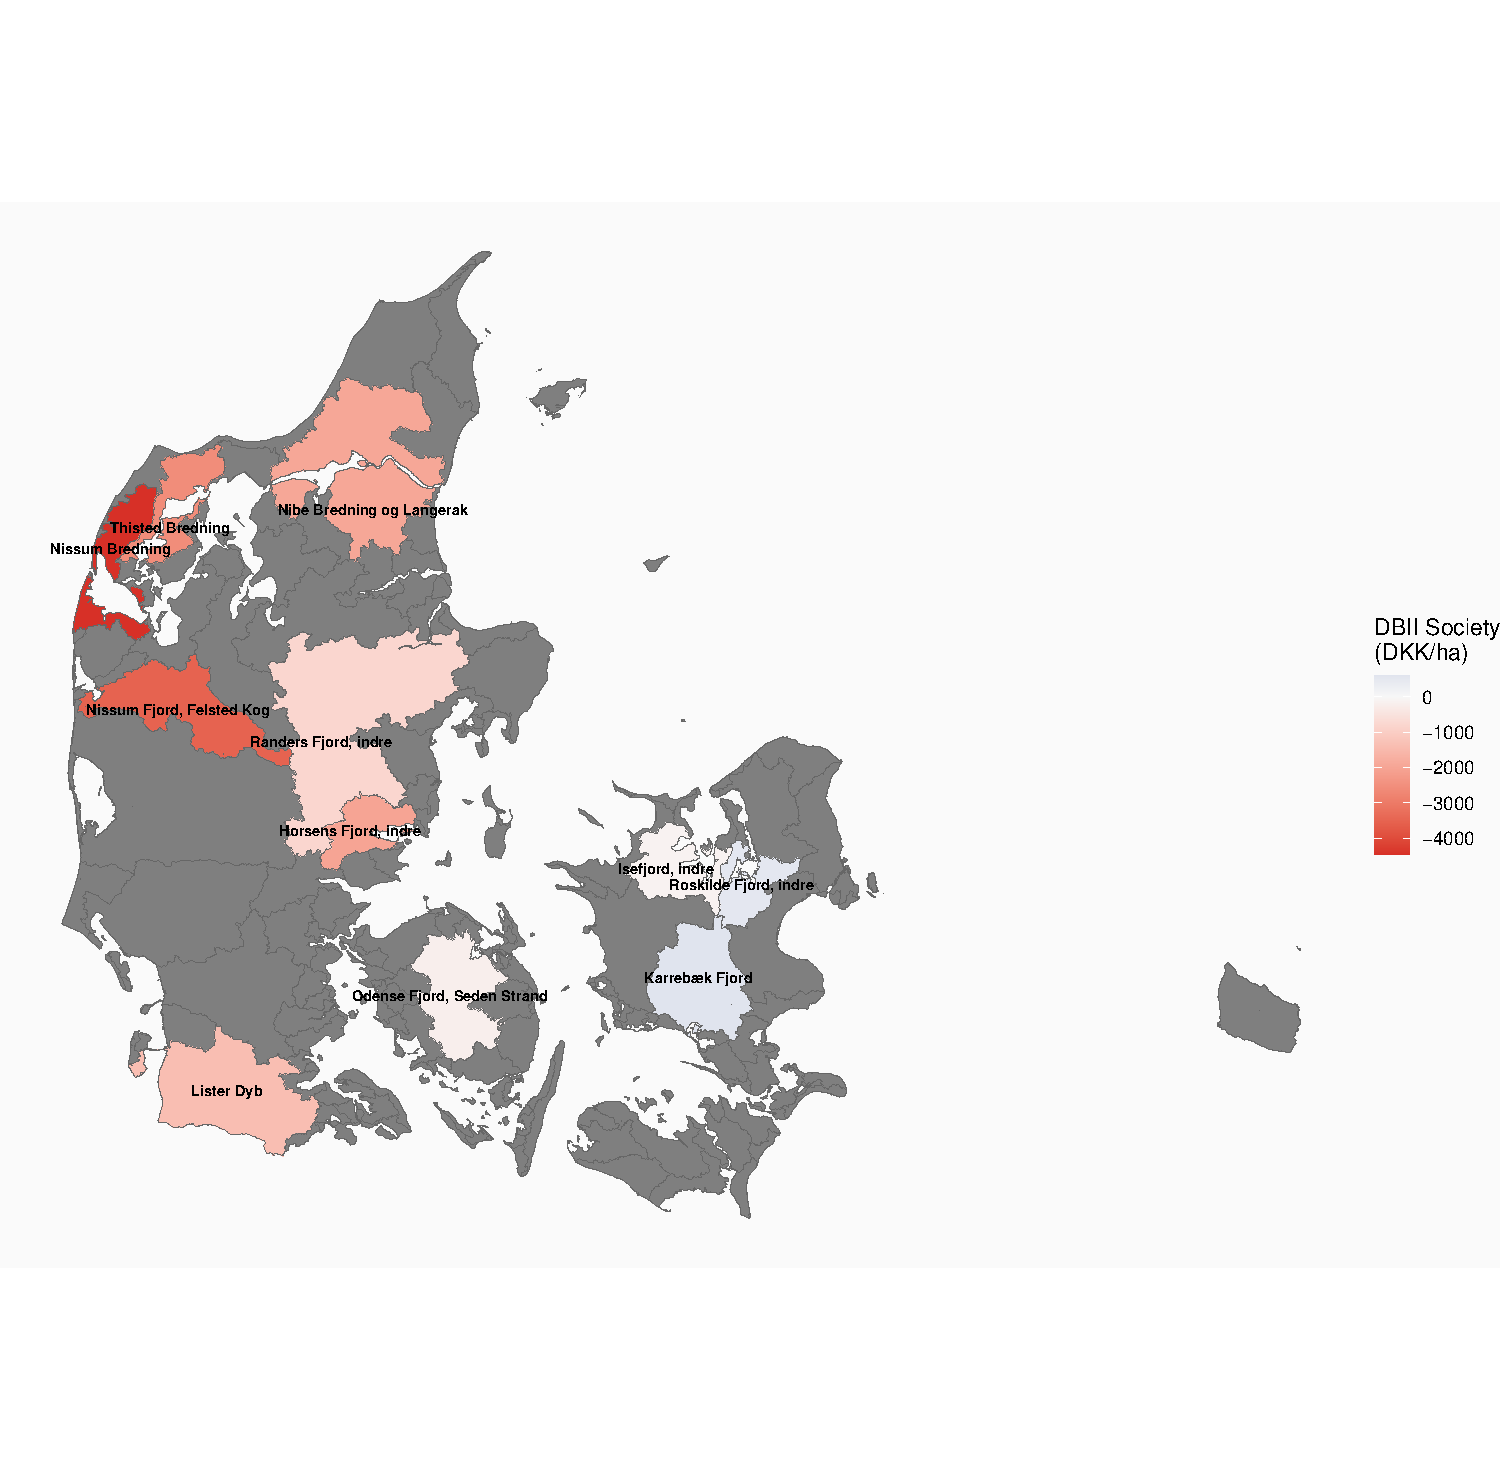
\includegraphics[width=\textwidth,height=1.2\textheight,keepaspectratio]{pictures/uniform.pdf}

\end{frame}


\begin{frame}[hvid]
\frametitle{\vspace{-3ex}C. Results: Field-Level Social Profitability (Uniform Approach)}
\centering
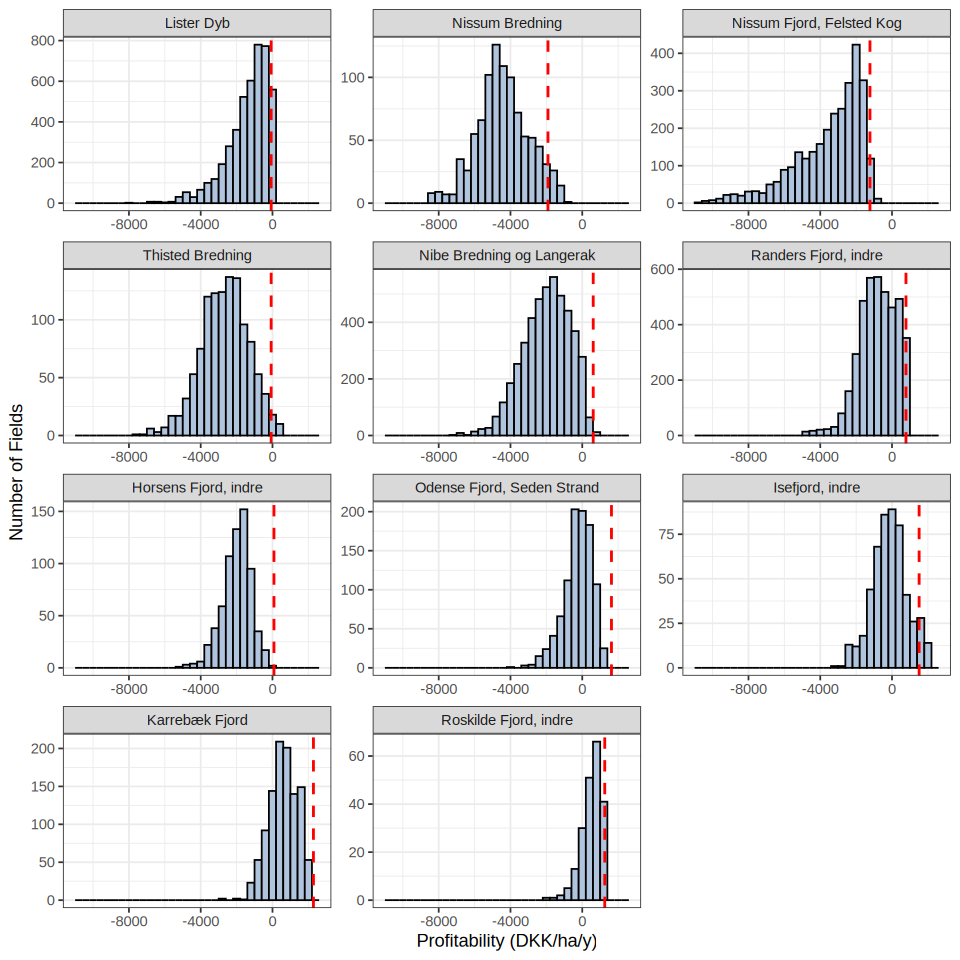
\includegraphics[width=\textwidth,height=0.8\textheight,keepaspectratio]{pictures/hist_uniform_DBII_hvede.png}

\end{frame}



\begin{frame}[hvid]
\frametitle{\vspace{-3ex}C. Results: Average Farmer Profitability (Spring Barley)}
\vspace{-1.6cm}
\centering
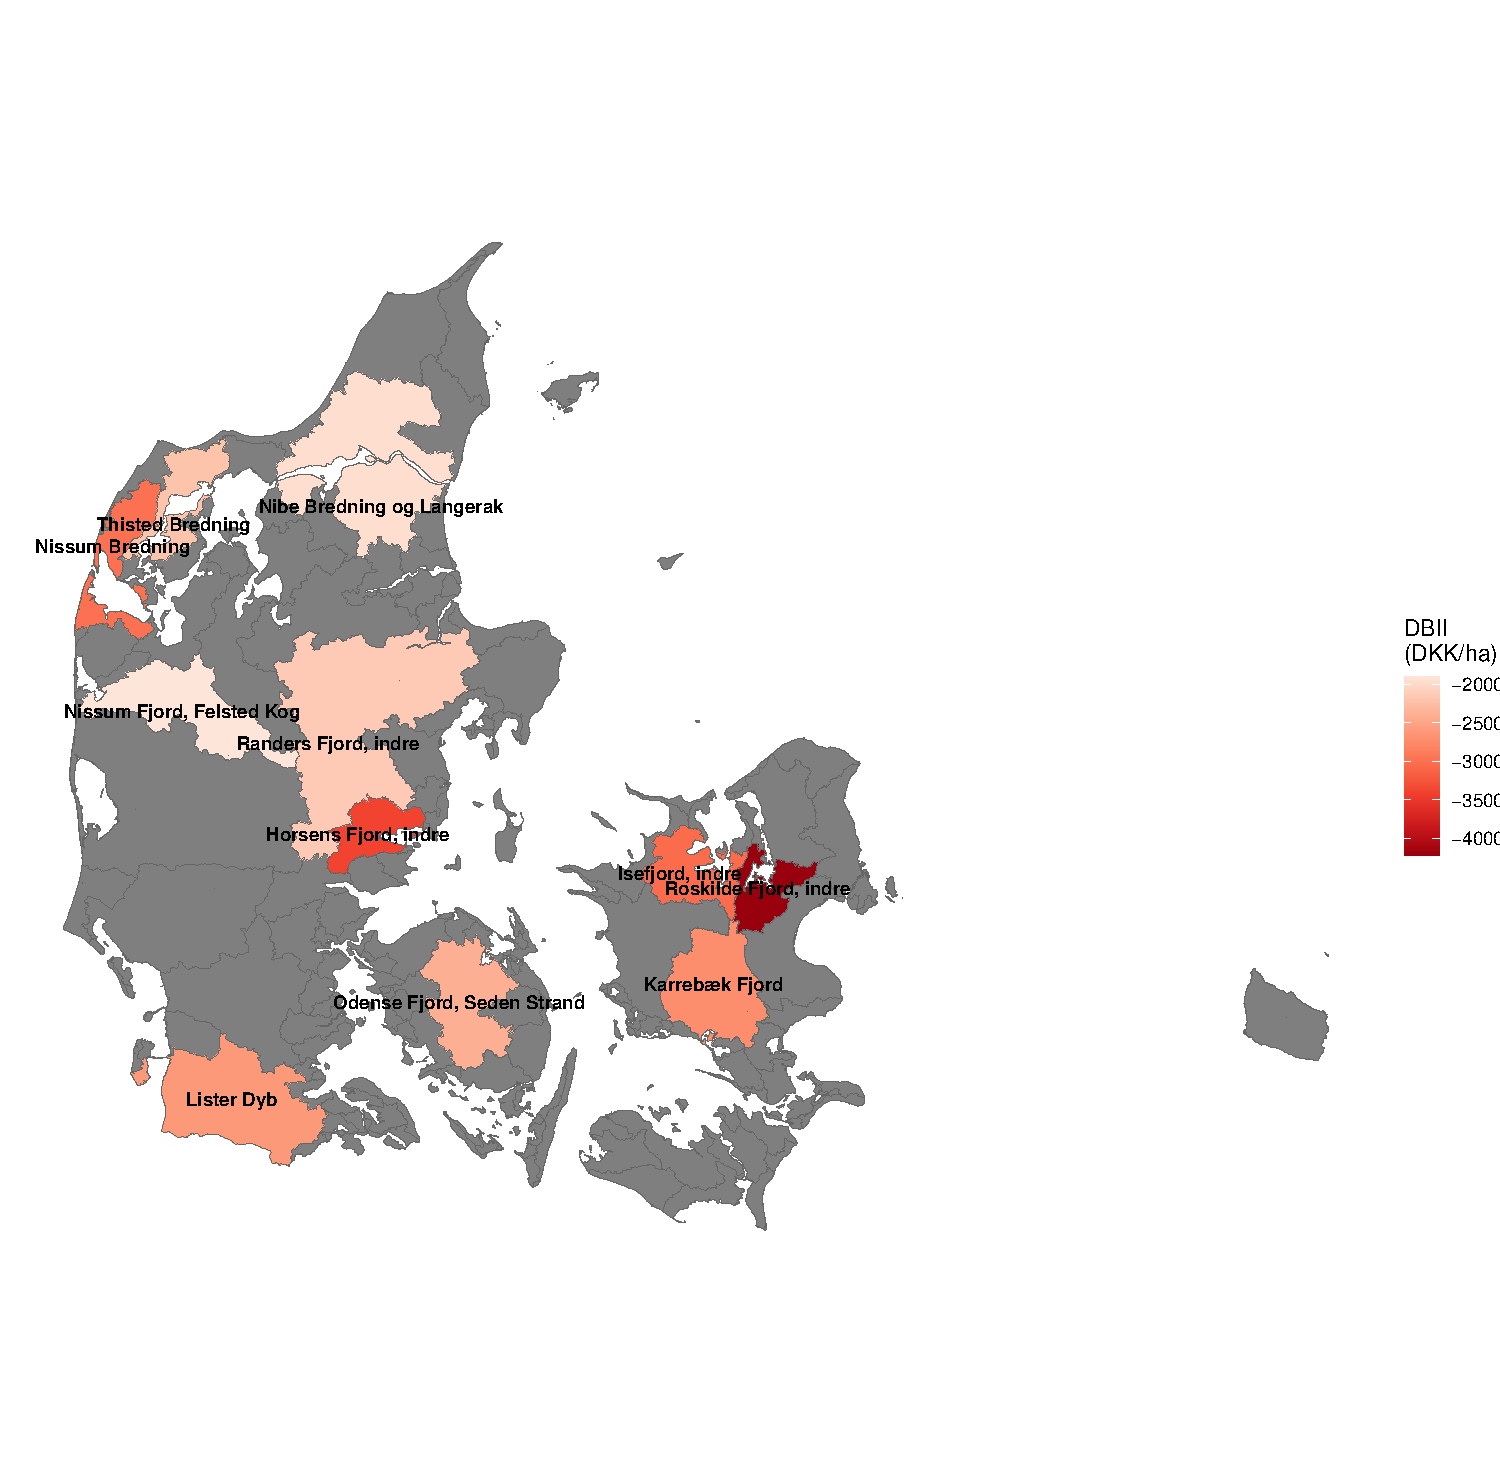
\includegraphics[width=\textwidth,height=1.2\textheight,keepaspectratio]{pictures/DBII_SB.pdf}

\end{frame}



\begin{frame}[hvid]
\frametitle{\vspace{-3ex}References}
\begin{itemize}
\item Andersen, M. S., Levin, G., and Odgaard, M. V. (2019). Economic benefits of reducing agricultural nitrogen losses to coastal waters for seaside recreation and real estate value in denmark. Marine Pollution Bulletin, 140:146–156.
\vspace{1ex}

\item Brink, C., van Grinsven, H., Jacobsen, B. H., and Velthof, G. (2011). Costs and benefits of nitrogen in the environment. In Sutton, M. A., Howard, C. M., Erisman, J. W., Billen, G., Bleeker, A., Grennfelt, P., van Grinsven, H., and Grizzetti, B., editors, The European Nitrogen Assessment. Cambridge University Press, Cambridge.
\vspace{1ex}

\item Henningsen, A., Zitthen, R. S., Andreasen, S. A., Frandsen, M., Jürgensen, M. S., and Vissing, W. L. R. (2026). Estimating input allocation coefficients from aggregate firm-level data. Unpublished document.
\end{itemize}
\end{frame}


\end{document}